\chapter{量化}
\label{chap:quantization}

一个传感器读出的是实数，例如某个零件尺寸偏离标称值的毫米数。它服从密度为$f(x)=\tfrac12\mathrm{e}^{-\lvert x\rvert}$的Laplace分布$\operatorname{Laplace}(0,1)$：多数读数靠近零，偶尔出现较大的偏差。若每个读数只允许存2个比特，也就是只能记录4种结果之一，那么这4个代表值应当放在哪里？哪些读数归给哪个代表值？这样记录后，平均要付出多大的平方误差？

第~\ref{chap:lossless-coding}章要求接收者精确还原每个符号。连续取值做不到这一点：实数轴的任意一个区间里都有不可数多个数，而有限长的二进制串一共只有可数多个，任何有限描述都必须把许多不同的读数合并成同一个结果。合并会带来误差，问题变成在给定的描述资源下怎样合并，使误差尽量小。

本章先把这件事写成模型：把取值空间分成有限个区域，每个区域配一个重构值，再用源分布和失真函数计算平均代价，并分清点数、定长索引和压缩后索引长度这三种资源。随后构造标量量化器：等距划分最容易实现，按分布调整的划分则由“固定区域选代表、固定代表选区域”的交替改进得到。

接着把同样的两条条件推广到向量，说明联合码本怎样利用分量之间的相关性和区域形状，又要付出怎样的存储与搜索代价。量化器确定以后，区域索引是一个离散随机变量，可以用上一章的方法再压缩，这一步改变平均描述长度而不改变重构结果；若要把码长也一起优化，目标函数就要改写。最后分析误差本身：有限范围造成的过载、范围内的舍入，以及加入共享随机扰动之后误差与输入的关系怎样改变。

全章以上述Laplace读数为贯穿例子，多数数值可以手算。所用的期望、条件期望与方差分解来自第~\ref{chap:random-variable-moments}章和第~\ref{chap:conditional-expectation}章，熵与平均码长来自第~\ref{chap:information-measures}章和第~\ref{chap:lossless-coding}章。本章对数以$2$为底，描述长度以bit计。

\section{量化模型}
\label{sec:quant-model}

记录一个连续读数，最朴素的做法是规定一组刻度，把读数报成离它最近的刻度。温度计只标到$0.1$度，读数$20.03$和$20.04$都记成$20.0$。这已经包含了量化的全部要素：哪些读数被合并到一起，合并后报出哪个值，合并造成多大的差。下面先把这三件事分开写成数学对象，再规定怎样计算平均误差、怎样计量所用的描述资源。

\paragraph{区域、索引与重构值}

可以把量化想成把读数装进有限个抽屉：每个抽屉占取值空间的一块区域，读数落进哪块区域就放进哪个抽屉；记录时只写抽屉的编号，取用时每个编号对应一个事先约定的代表值。与温度计刻度不同，抽屉的边界和代表值都由我们来选，代表值也不必位于区域的正中。这个类比在一处会失效：抽屉里的东西还能取出来，而量化后只剩编号，同一区域内的不同读数已经无法区分。

取值空间记为$\mathbb{R}^{d}$，$d=1$是单个读数，$d\geq2$是几个读数一起处理。区域要能计算概率，所以要求它们是Borel集；在第~\ref{chap:probability-spaces}章的意义下，这保证了$\mathbb{P}(\bm{X}\in S_j)$有定义。

\begin{definition}[量化器]
\label{def:quant-quantizer}
设$N\geq1$为整数。取值空间$\mathbb{R}^{d}$上的一个$N$点\term{量化器}（quantizer）$Q$由两部分组成：一组两两不交、并集为$\mathbb{R}^{d}$的Borel集$S_1,\dots,S_N$，称为它的区域；以及$N$个点$\bm{c}_1,\dots,\bm{c}_N\in\mathbb{R}^{d}$，称为\term{重构值}（reconstruction value），全体$\mathcal{C}=\{\bm{c}_1,\dots,\bm{c}_N\}$称为\term{码本}（codebook）。编码器与解码器分别是
\begin{equation}
 \alpha(\bm{x})=j\quad(\bm{x}\in S_j),\qquad \beta(j)=\bm{c}_j ,
 \label{eq:quant-encoder-decoder}
\end{equation}
量化器是二者的复合$Q(\bm{x})=\beta(\alpha(\bm{x}))$。
\end{definition}

编码器$\alpha$只输出区域的编号，称为\term{量化索引}（quantization index）；解码器$\beta$只看编号，不知道原来的读数。因此$Q$在每个区域上取常值，它的值域至多有$N$个点。对随机输入$\bm{X}$，索引$J=\alpha(\bm{X})$是取值于$\{1,\dots,N\}$的离散随机变量，概率质量为
\begin{equation}
 p_j=\mathbb{P}(J=j)=\mathbb{P}(\bm{X}\in S_j),\qquad j=1,\dots,N .
 \label{eq:quant-index-pmf}
\end{equation}

区域之间的边界点归哪一侧，需要事先约定。对有密度的输入，边界通常是概率为零的集合，约定不影响平均误差；对离散输入，边界上可能有正的概率，约定会改变结果，后面遇到时再说明。

\paragraph{失真与平均失真}

合并的代价用一个非负函数衡量：读数为$\bm{x}$而报出$\hat{\bm{x}}$时，代价是$d(\bm{x},\hat{\bm{x}})\geq0$，称为\term{失真函数}（distortion function），要求它是Borel可测的。本章主要使用平方误差
\begin{equation}
 d(\bm{x},\hat{\bm{x}})=\lVert\bm{x}-\hat{\bm{x}}\rVert_2^2 ,
 \label{eq:quant-squared-error}
\end{equation}
标量情形就是$(x-\hat{x})^2$。平方误差对大偏差惩罚更重，并且能和期望、方差的运算直接配合，下一节会反复用到这一点。

单个读数的失真是随机的，评价量化器时取它的平均。

\begin{definition}[平均失真]
\label{def:quant-average-distortion}
设$\bm{X}$的分布为$P_{\bm{X}}$，$Q$是由区域$S_j$和重构值$\bm{c}_j$给出的量化器。$Q$的\term{平均失真}（average distortion）是
\begin{equation}
 D(Q)=\mathbb{E}\bigl[d(\bm{X},Q(\bm{X}))\bigr]=\sum_{j=1}^{N}\int_{S_j}d(\bm{x},\bm{c}_j)\,P_{\bm{X}}(\mathrm{d}\bm{x}) .
 \label{eq:quant-average-distortion}
\end{equation}
它是非负可测函数的期望，总有定义，可能为$+\infty$。
\end{definition}

式~\eqref{eq:quant-average-distortion}的第二个等号把期望按区域拆开：在$S_j$上$Q$恒等于$\bm{c}_j$，所以每块只是一个普通的积分。对平方误差，只要$\mathbb{E}[\lVert\bm{X}\rVert_2^2]<\infty$，平均失真对任何码本都有限，因为
\[
 \lVert\bm{x}-\bm{c}_j\rVert_2^2\leq2\lVert\bm{x}\rVert_2^2+2\lVert\bm{c}_j\rVert_2^2 .
\]
本章讨论平方误差时都假定输入的二阶矩有限。

平均失真同时依赖三样东西：源分布、区域划分和重构值。源分布是给定的，后两者由设计者选择。“好的量化器”永远是相对于某个源分布和某个失真函数而言的，换一个分布，同一个量化器的平均失真就会改变。

\paragraph{两点量化器}
用本章开头的Laplace读数$X\sim\operatorname{Laplace}(0,1)$走一遍。只允许两个重构值时，按符号分成两个区域，配上对称的两个点：
\[
 S_1=(-\infty,0),\quad S_2=[0,\infty),\qquad c_1=-1,\quad c_2=1 .
\]
例如读数$x=0.7$落在$S_2$，编码器输出$j=2$，解码器报出$c_2=1$，误差是$0.3$。

计算平均失真时，由对称性，两个区域贡献相同，只需算$S_2$。在$X\geq0$的条件下，$X$服从$\operatorname{Exp}(1)$，第~\ref{chap:common-distributions}章给出它的一、二阶矩
\[
 \mathbb{E}[X\mid X\geq0]=1,\qquad \mathbb{E}[X^{2}\mid X\geq0]=2 .
\]
把平方展开，得到
\[
 \mathbb{E}\bigl[(X-1)^{2}\mid X\geq0\bigr]=2-2\cdot1+1=1 .
\]
两个区域各占概率$\tfrac12$，于是
\[
 D(Q)=\tfrac12\cdot1+\tfrac12\cdot1=1 .
\]

作为对照，如果什么都不记录，只能对所有读数报同一个常数$c$。平方误差$\mathbb{E}[(X-c)^2]$在$c=\mathbb{E}[X]=0$时最小，最小值是$\operatorname{Var}(X)=2$。一个比特把平均失真从$2$降到$1$。图~\ref{fig:quant-two-points}画出了这个量化器：左图是两个区域与重构值在密度上的位置，右图是映射$Q(x)$本身，它是一条只取两个值的阶梯，与对角线$y=x$的竖直距离就是误差。

\begin{BookInlineFigure}
 \centering
 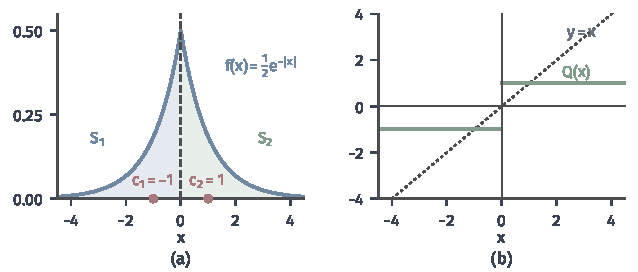
\includegraphics[width=108mm]{figures/07-probability/05-source-coding/matplotlib/quant-two-points/figure.pdf}
 \caption{$\operatorname{Laplace}(0,1)$读数的两点量化器。(a) 蓝线为密度$f$，浅蓝与浅绿分别是区域$S_1=(-\infty,0)$与$S_2=[0,\infty)$，红点为重构值$c_1=-1$、$c_2=1$，虚线为区域边界。(b) 绿线为$Q(x)$，点线为$y=x$；同一横坐标处二者的竖直距离就是误差。}
 \label{fig:quant-two-points}
\end{BookInlineFigure}

最好的重构值依赖于失真函数。若改用绝对误差$d(x,\hat{x})=\lvert x-\hat{x}\rvert$，一个区域内最好的代表值不再是条件均值，而是条件中位数：均值使平方误差最小，中位数使绝对误差最小。在$X\geq0$的条件下，$\operatorname{Exp}(1)$的中位数是$\ln2\approx0.693$，对$Z\sim\operatorname{Exp}(1)$与$c\geq0$直接积分得
\[
 \mathbb{E}\lvert Z-c\rvert=c-1+2\mathrm{e}^{-c} .
\]
取$c=\ln2$得平均绝对误差$0.693$，取$c=1$得$0.736$。同一个源、同样的两个区域，换一个失真函数，最好的重构值就从$\pm1$移到了$\pm0.693$。

右图也显示了误差的两个特点。读数靠近$\pm1$时误差小，远离时误差随$\lvert x\rvert$线性增长；误差完全由读数决定，没有任何随机性。第~\ref{sec:quant-error}节会专门分析这两点。

\paragraph{描述资源}

量化减少了需要记录的内容，但“减少了多少”有三种不同的计量方法，混用会得出错误的比较。图~\ref{fig:quant-pipeline}把一次记录拆成几个环节：编码器把读数变成索引，索引可以原样写成定长比特串，也可以先经过一次无损编码再传送，接收端恢复索引后由解码器报出重构值。

\begin{BookInlineFigure}
 \centering
 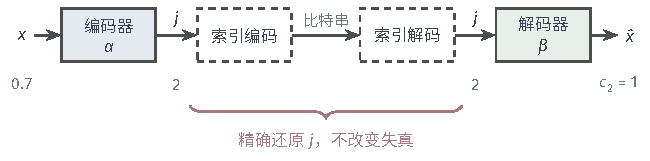
\includegraphics[width=110.1mm]{figures/07-probability/05-source-coding/tikz/quant-pipeline/figure.pdf}
 \caption{量化记录的各个环节。实线框是量化器本身：编码器$\alpha$输出区域索引$j$，解码器$\beta$报出重构值；虚线框是可选的索引编码与解码。下方灰字是两点量化器的例子：读数$0.7$得到索引$2$，重构为$c_2=1$。中间两个环节精确还原索引，因此不改变失真。}
 \label{fig:quant-pipeline}
\end{BookInlineFigure}

第一种计量是重构点数$N$，它决定量化器能区分多少种结果。第二种是\emph{定长索引长度}：每个索引都用同样多的比特写出，需要$\lceil\log_2N\rceil$个比特；$N$是$2$的幂时恰为$\log_2N$。第三种是\emph{平均索引长度}：把索引$J$看作一个离散信源，用第~\ref{chap:lossless-coding}章的唯一可译码描述它，平均长度不小于索引的熵
\[
 H(J)=-\sum_{j=1}^{N}p_j\log_2p_j ,
\]
又可以做到小于$H(J)+1$。由于$H(J)\leq\log_2N$，平均索引长度可以明显短于定长索引长度，尤其当各区域的概率很不均匀时。

处理向量时还要说清是按什么计算的。$d$个读数组成一个向量、用$N$个重构点描述时，每个向量用$\log_2N$个比特，折合每个分量
\begin{equation}
 R=\frac{1}{d}\log_2N
 \label{eq:quant-rate-per-component}
\end{equation}
个比特。比较一个标量量化器和一个二维量化器时，应当在相同的每分量比特数下比较，而不是在相同的点数下比较。

\begin{BookInlineTable}
 \centering
 \begin{tabular}{lll}
  \toprule
  资源 & 计量 & 两点量化器\\
  \midrule
  重构点数 & $N$ & $2$\\
  定长索引长度 & $\lceil\log_2N\rceil$ & $1$ bit\\
  平均索引长度 & 不小于$H(J)$ & $1$ bit\\
  \bottomrule
 \end{tabular}
 \caption{三种描述资源。两点量化器的两个区域概率都是$\tfrac12$，三种计量恰好一致；区域概率不均匀时，平均索引长度可以小于定长索引长度。}
 \label{tab:quant-resources}
\end{BookInlineTable}

表~\ref{tab:quant-resources}汇总了这三种计量。它们回答不同的问题：点数决定重构的精细程度，定长长度适合每个读数必须占用固定存储的场合，平均长度适合可以变长记录的场合。第~\ref{sec:quant-index-coding}节将看到，固定点数时用变长记录可以节省长度，而若以平均长度为预算，最优的区域划分也会随之改变。

\paragraph{有限量化器与长块极限}

给定源分布、失真函数、维数$d$和点数$N$，所有$N$点量化器中平均失真的下确界
\[
 D_N^{*}=\inf_{Q:\,N\text{点}}D(Q)
\]
是有限量化所能达到的最好水平。它依赖于一次联合处理多少个读数。同样是每个读数1 bit，逐个读数用两点量化器，与把两个读数作为二维向量用四点量化器，后者的选择范围包含前者（取两个两点量化器的乘积即可），因此不会更差，往往还更好；第~\ref{sec:quant-vector}节会给出具体例子。

把越来越长的读数块放在一起描述，每分量的最低失真还会继续下降。第~\ref{chap:rate-distortion}章研究这一极限：对方差为$\sigma^{2}$的高斯读数，允许任意长的块时，每个读数1 bit可以把均方误差降到$\sigma^{2}/4$，而逐个读数的最好两点量化器（阈值为零、重构值为$\pm\sigma\sqrt{2/\pi}$）只能达到$(1-2/\pi)\sigma^{2}\approx0.363\sigma^{2}$。所以本章算出的有限量化器失真，是具体方案在给定维数和点数下的表现，不等于给定码率下所有长块编码的最小失真；两者的差距正是下一章要衡量的量。


\section{标量量化}
\label{sec:quant-scalar}

先处理单个实值读数，$d=1$。实轴上最自然的区域是区间：取阈值
\[
 -\infty=t_0<t_1<\dots<t_{N-1}<t_N=+\infty ,
\]
令$S_j=[t_{j-1},t_j)$，再在每个区间里放一个重构值$c_j$。编码器只要把读数与阈值逐个比较，就能确定它落在哪个区间。这样的量化器称为\term{标量量化}（scalar quantization）。

区间怎么划、重构值放在哪里，有两种思路。一种是不看分布，直接按等距刻度划分，构造和编码都最简单；另一种是按源分布调整，概率集中的地方划得细，稀疏的地方划得粗。对平方误差，后一种思路可以拆成两个各自容易求解的子问题：区间固定时重构值放在哪里最好，重构值固定时区间边界放在哪里最好。轮流求解这两个子问题，就得到第~\ref{sec:quant-nonuniform}节的迭代。

\subsection{均匀量化}
\label{sec:quant-uniform}

等距划分需要先规定三件事：表示范围$[-L,L]$、重构点数$N$，以及范围外的读数怎样处理。范围被等分为$N$段，步长为
\[
 \Delta=\frac{2L}{N} .
\]

\paragraph{区间与重构值}
第$j$段区间的左右端点是$-L+(j-1)\Delta$和$-L+j\Delta$，重构值取它的中点。内部阈值和重构值分别为
\begin{equation}
 t_j=-L+j\Delta\ (j=1,\dots,N-1),\qquad c_j=-L+\bigl(j-\tfrac12\bigr)\Delta\ (j=1,\dots,N).
 \label{eq:quant-uniform-points}
\end{equation}
范围外的读数归入最外侧的区间：$x<-L$报$c_1$，$x\geq L$报$c_N$。这种约定称为\term{饱和}（saturation），相当于把两端的区间延长到无穷。于是编码器可以写成一个公式，
\begin{equation}
 \alpha(x)=\min\Bigl\{N,\ \max\Bigl\{1,\ \Bigl\lfloor\frac{x+L}{\Delta}\Bigr\rfloor+1\Bigr\}\Bigr\} ,
 \label{eq:quant-uniform-encoder}
\end{equation}
内层的取整给出读数在第几段，外层的$\max$与$\min$实现饱和。解码器按式~\eqref{eq:quant-uniform-points}查出$c_{\alpha(x)}$。这样构造的量化器称为\term{均匀量化}（uniform quantization）。

式~\eqref{eq:quant-uniform-points}中相邻重构值的中点恰好是阈值，所以在每个读数处，均匀量化器报出的都是离它最近的重构值。点数$N$为偶数时，零是阈值而不是重构值，读数在零附近时报$\pm\Delta/2$；若希望零本身是重构值，可以把刻度平移半个步长，取$c=k\Delta$，这样的量化器在第~\ref{sec:quant-dither}节使用。

\paragraph{一个编码与重构的例子}
取$N=8$、$L=4$，步长$\Delta=1$，重构值为$\pm0.5,\pm1.5,\pm2.5,\pm3.5$，每个索引用$3$个比特。下面检验三个读数。

读数$x=1.3$在范围内，$\lfloor5.3\rfloor+1=6$，于是
\[
 \alpha(1.3)=6,\qquad Q(1.3)=c_6=-4+5.5=1.5 ,
\]
误差为$0.2$。读数$x=-0.2$同样在范围内，$\lfloor3.8\rfloor+1=4$，
\[
 \alpha(-0.2)=4,\qquad Q(-0.2)=c_4=-0.5 ,
\]
误差为$-0.3$。

读数$x=5.7$超出了范围。$\lfloor9.7\rfloor+1=10$，被$\min$截到$8$，
\[
 \alpha(5.7)=8,\qquad Q(5.7)=c_8=3.5 ,
\]
误差为$-2.2$，远大于半个步长。图~\ref{fig:quant-uniform-staircase}把$Q$画成阶梯，三个读数的误差是红色竖线的长度。

\begin{BookInlineFigure}
 \centering
 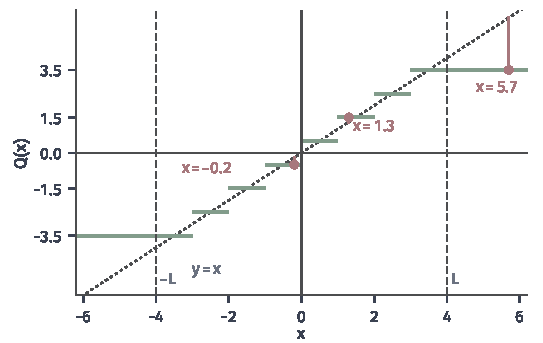
\includegraphics[width=92mm]{figures/07-probability/05-source-coding/matplotlib/quant-uniform-staircase/figure.pdf}
 \caption{$N=8$、$L=4$、$\Delta=1$的均匀量化器。绿线为阶梯$Q(x)$，点线为$y=x$，虚线标出表示范围的两端。红点是读数$1.3$、$-0.2$、$5.7$的输出，红色竖线的长度是误差；范围外的阶梯无限延长，误差随读数线性增大。}
 \label{fig:quant-uniform-staircase}
\end{BookInlineFigure}

\paragraph{有限范围的两种误差}
图中可以分出两种情形。读数在$[-L,L]$内时，它与所在区间的中点相距不超过半个步长，
\[
 \lvert x-Q(x)\rvert\leq\frac{\Delta}{2},\qquad \lvert x\rvert\leq L ;
\]
这部分误差称为\term{舍入误差}（granular error）。读数超出范围时，误差为$\lvert x\rvert-(L-\Delta/2)$，随读数无限增大，称为\term{过载误差}（overload error）。

只要$N$有限而区间都有界，就覆盖不了整条实轴，总要对范围外的读数作某种约定。饱和是最简单的一种。另一种做法是保留一个“越界”索引，再另外描述越界的读数，这等于增加了点数或改变了索引长度，比较时要把这部分资源计入。

两种误差对步长的要求相反。$N$固定时，缩小步长使舍入误差变小，却使范围$L=N\Delta/2$变窄、过载更频繁。对Laplace读数取$N=4$、$\Delta=1$，即$L=2$，重构值为$\pm0.5,\pm1.5$，平均失真为$0.5142$；第~\ref{sec:quant-granular-overload}节将把它分解成两部分，并给出权衡的方法。这个四点量化器也是下一小节迭代的起点。

\subsection{非均匀量化}
\label{sec:quant-nonuniform}

Laplace读数集中在零附近，尾部却延伸得很远。均匀刻度在这里有些浪费：中间密集的地方和尾部稀疏的地方用同样的步长。直观上，概率大的地方应当划得细些，概率小的地方划得粗些。下面固定点数$N$和平方误差，寻找使平均失真最小的区间和重构值。这样构造的量化器一般不等距，称为\term{非均匀量化}（non-uniform quantization）。

同时优化$N-1$个阈值和$N$个重构值并不容易，因为目标对它们的依赖相互纠缠。把变量分成两组，每次固定一组优化另一组，两个子问题都有显式解。

\paragraph{固定区间选重构值}
区间固定后，平均失真按区间拆成互不相关的几块，每块只依赖一个重构值，可以分别优化。于是问题化为：在一个区间上放一个点，使该区间内的平方误差最小。

期望是质量分布的重心，方差是绕重心的转动惯量。把区间$S$上的那部分概率质量看作一块物体，平方误差$\mathbb{E}[(X-c)^2\mathbf{1}_{\{X\in S\}}]$就是它绕点$c$的转动惯量，最好的$c$应当是这块质量的重心。下面的引理把这个直观写成恒等式，它是力学中平行轴定理的概率版本。

\begin{lemma}[质心条件]
\label{lem:quant-centroid}
设$\mathbb{E}[X^{2}]<\infty$，$S$是Borel集且$p=\mathbb{P}(X\in S)>0$，记条件均值
\begin{equation}
 m=\mathbb{E}[X\mid X\in S]=\frac{\mathbb{E}[X\mathbf{1}_{\{X\in S\}}]}{p} .
 \label{eq:quant-conditional-mean}
\end{equation}
则对每个实数$c$，
\begin{equation}
 \mathbb{E}\bigl[(X-c)^{2}\mathbf{1}_{\{X\in S\}}\bigr]=\mathbb{E}\bigl[(X-m)^{2}\mathbf{1}_{\{X\in S\}}\bigr]+p\,(m-c)^{2} .
 \label{eq:quant-parallel-axis}
\end{equation}
因此该区间内的平方误差在$c=m$时唯一地取到最小。
\end{lemma}

\begin{proof}
把$X-c$写成$(X-m)+(m-c)$，平方后展开：
\[
 (X-c)^{2}=(X-m)^{2}+2(m-c)(X-m)+(m-c)^{2} .
\]
两边乘$\mathbf{1}_{\{X\in S\}}$再取期望。二阶矩有限保证每一项都可积。交叉项中，
\[
 \mathbb{E}\bigl[(X-m)\mathbf{1}_{\{X\in S\}}\bigr]=\mathbb{E}[X\mathbf{1}_{\{X\in S\}}]-mp=0 ,
\]
最后一步用了式~\eqref{eq:quant-conditional-mean}。常数项的期望是$p(m-c)^{2}$，于是得到式~\eqref{eq:quant-parallel-axis}。右边第一项与$c$无关，第二项非负且只在$c=m$时为零，所以最小点唯一。
\end{proof}

式~\eqref{eq:quant-parallel-axis}说明，重构值偏离重心的代价是区间概率乘以偏离距离的平方，且与区间内部的分布形状无关。满足这一条件的重构值称为区间的质心。

用第~\ref{chap:conditional-expectation}章的语言，若每个正概率区间的重构值都是质心，则$Q(X)=\mathbb{E}[X\mid J]$，即量化输出是读数在“只知道索引”这一信息下的条件期望，也就是$X$到索引所生成的信息上的正交投影。正交性给出一个计算平均失真的捷径：
\begin{equation}
 D(Q)=\mathbb{E}[X^{2}]-\mathbb{E}\bigl[Q(X)^{2}\bigr]=\mathbb{E}[X^{2}]-\sum_{j=1}^{N}p_jc_j^{2} .
 \label{eq:quant-centroid-distortion}
\end{equation}
它由勾股定理
\[
 \mathbb{E}[X^{2}]=\mathbb{E}\bigl[Q(X)^{2}\bigr]+\mathbb{E}\bigl[(X-Q(X))^{2}\bigr]
\]
得到，只在重构值都是质心时成立。

以Laplace读数为例，看区间$[0,1)$。按$\operatorname{Laplace}(0,1)$的密度直接积分，得到这个区间的概率与一阶矩：
\[
 p=\frac{1-\mathrm{e}^{-1}}{2}=0.3161,\qquad \mathbb{E}[X\mathbf{1}_{\{0\leq X<1\}}]=\frac{1-2\mathrm{e}^{-1}}{2}=0.1321 .
\]
二者相除，质心为
\[
 m=\frac{0.1321}{0.3161}=0.4180 .
\]
它比区间中点$0.5$更靠近零，因为密度在区间内向右递减，质量偏向左端。图~\ref{fig:quant-centroid-nn}左图画出该区间内的平方误差随$c$变化的抛物线：最低点在$m=0.418$，中点$0.5$处的值比最低点多出$p(0.5-0.418)^2=0.0021$。

\begin{BookInlineFigure}
 \centering
 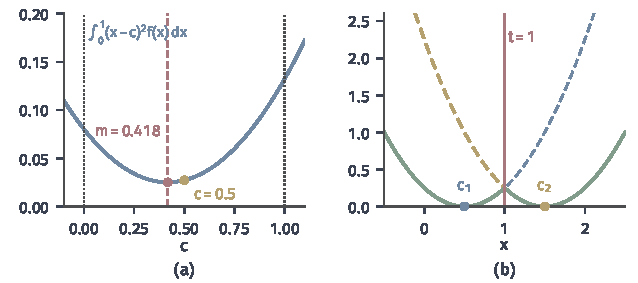
\includegraphics[width=108mm]{figures/07-probability/05-source-coding/matplotlib/quant-centroid-nn/figure.pdf}
 \caption{两个子问题的解。(a) $\operatorname{Laplace}(0,1)$在区间$[0,1)$上的平方误差$\int_0^1(x-c)^2f(x)\,\mathrm{d}x$随$c$的变化（蓝线），最低点在质心$m=0.418$（红点），区间中点$c=0.5$（黄点）处略高。(b) 固定重构值$c_1=0.5$、$c_2=1.5$时，两条虚线是$(x-c_1)^2$与$(x-c_2)^2$，绿线是它们的下包络；两者在中点$t=1$（红线）处交换。}
 \label{fig:quant-centroid-nn}
\end{BookInlineFigure}

\paragraph{固定重构值选区间}
现在反过来，重构值$c_1<\dots<c_N$固定，问每个读数应归入哪个区间。平均失真是逐点误差的期望，而逐点误差只取决于这个读数被报成哪个值。所以对每个读数分别选最近的重构值，就使平均失真最小，不需要考虑其他读数。

\begin{lemma}[最近邻条件]
\label{lem:quant-nearest}
设重构值$c_1,\dots,c_N$固定，$Q$是以它们为重构值的任一量化器。则
\begin{equation}
 D(Q)\geq\mathbb{E}\Bigl[\min_{1\leq k\leq N}(X-c_k)^{2}\Bigr] ,
 \label{eq:quant-nearest-bound}
\end{equation}
等号成立当且仅当以概率$1$有$(X-Q(X))^{2}=\min_k(X-c_k)^{2}$，即几乎每个读数都被报成离它最近的重构值。
\end{lemma}

\begin{proof}
对每个$x$，$Q(x)$是某个$c_k$，所以逐点有$(x-Q(x))^{2}\geq\min_k(x-c_k)^{2}$。两边是非负可测函数，取期望即得式~\eqref{eq:quant-nearest-bound}。两边之差是非负随机变量，它的期望为零当且仅当它几乎必然为零，这就是等号条件。
\end{proof}

最近邻规则下的区间可以直接算出来。对相邻的两个重构值，比较两种误差：
\[
 (x-c_j)^{2}-(x-c_{j+1})^{2}=(c_{j+1}-c_j)\bigl(2x-c_j-c_{j+1}\bigr) .
\]
由于$c_{j+1}>c_j$，左边小于零当且仅当$x$小于两点的中点。所以最近邻区间仍是区间，阈值是相邻重构值的中点：
\begin{equation}
 t_j=\frac{c_j+c_{j+1}}{2},\qquad j=1,\dots,N-1 .
 \label{eq:quant-midpoint-threshold}
\end{equation}
读数恰好落在中点时两个重构值一样近，需要约定归属，例如归入编号较小的一个。对有密度的读数，中点的概率为零，约定不影响平均失真。图~\ref{fig:quant-centroid-nn}右图画出两条误差抛物线和它们的下包络，交点就在中点$t=1$。

\paragraph{两条必要条件}
两个引理合起来，就是最优量化器必须满足的条件。

\begin{theorem}[Lloyd--Max条件]
\label{thm:quant-lloyd-max-conditions}
设$\mathbb{E}[X^{2}]<\infty$，平方误差下$Q^{*}$在所有$N$点量化器中平均失真最小，其区间为$S_j$、重构值为$c_j$。则：
\begin{enumerate}
 \item 对每个$p_j=\mathbb{P}(X\in S_j)>0$，$c_j=\mathbb{E}[X\mid X\in S_j]$；
 \item 以概率$1$有$(X-c_{\alpha(X)})^{2}=\min_k(X-c_k)^{2}$。
\end{enumerate}
\end{theorem}

\begin{proof}
若第一条对某个$j$不成立，由引理~\ref{lem:quant-centroid}，把$c_j$换成条件均值严格减小区间$S_j$上的误差，其余区间不变，平均失真严格下降，与$Q^{*}$最优矛盾。若第二条不成立，由引理~\ref{lem:quant-nearest}，保持重构值、按最近邻重新划分，平均失真严格下降，同样矛盾。
\end{proof}

这两条只是必要条件，不是充分条件：满足它们的量化器可能不是最优的，后面会给出例子。定理也没有断言最优量化器存在。对平方误差和二阶矩有限的读数，$N$点最优量化器确实存在：离分布太远的重构值可以拉回而不增大失真，于是只需在有界的重构值集合中寻找，再用紧性论证取到最小值。下面的迭代只用到两条必要条件，不依赖存在性。

\paragraph{交替改进的思想}
两条条件提示了一个迭代：从某组重构值出发，先按式~\eqref{eq:quant-midpoint-threshold}取中点作阈值，再按式~\eqref{eq:quant-conditional-mean}把每个重构值移到新区间的质心，然后重复。每一步都是在固定另一组变量时求得的最优解，所以平均失真不会上升。这种做法称为\term{Lloyd--Max算法}（Lloyd--Max algorithm）。写成公式，第$t$轮的两步为
\begin{equation}
 t_j^{(t)}=\frac{c_j^{(t-1)}+c_{j+1}^{(t-1)}}{2},\qquad
 c_j^{(t)}=\mathbb{E}\bigl[X\bigm| t_{j-1}^{(t)}\leq X<t_j^{(t)}\bigr] ,
 \label{eq:quant-lloyd-update}
\end{equation}
其中$t_0^{(t)}=-\infty$、$t_N^{(t)}=+\infty$。

对Laplace读数，质心有显式形式，迭代可以手算。$\operatorname{Laplace}(0,1)$在$x\geq0$上就是$\frac12\mathrm{e}^{-x}$，对$0\leq a<b$，积分得到区间的概率与条件均值：
\begin{equation}
 \begin{gathered}
 \mathbb{P}(a\leq X<b)=\frac{\mathrm{e}^{-a}-\mathrm{e}^{-b}}{2},\\
 \mathbb{E}[X\mid a\leq X<b]=\frac{(a+1)\mathrm{e}^{-a}-(b+1)\mathrm{e}^{-b}}{\mathrm{e}^{-a}-\mathrm{e}^{-b}} .
 \end{gathered}
 \label{eq:quant-laplace-centroid}
\end{equation}
令$b\to\infty$，得到$\mathbb{E}[X\mid X\geq a]=a+1$：超过$a$的部分服从$\operatorname{Exp}(1)$，均值为$1$，这是指数分布无记忆性的直接结果。负半轴由对称性得到。

\paragraph{计算过程}
下面用$N=4$、从上一小节的均匀量化器出发，逐轮演示。读数分布关于零对称，初始重构值也对称，每轮更新后仍对称，所以中间阈值始终为$0$，只需跟踪正半轴的一个阈值和两个重构值。

\needspace{6\baselineskip}
\paragraph{变量}
\begin{itemize}
 \item $c_1^{(t)}<\dots<c_N^{(t)}$：第$t$轮的重构值，共$N$个实数。
 \item $t_1^{(t)}<\dots<t_{N-1}^{(t)}$：第$t$轮的阈值，共$N-1$个实数，两端补$\pm\infty$。
 \item $D^{(t)}$：第$t$轮量化器的平均失真，用于判断何时停止。
\end{itemize}
例中由对称性，只需记录$t_3^{(t)}$、$c_3^{(t)}$与$c_4^{(t)}$。

\paragraph{初始化}
重构值初始化为一组互不相同的点，常用的选择是同样点数的均匀量化器，或者从源分布中抽取的几个值。$D^{(0)}$是这组点配上最近邻区间时的平均失真。例中取$\Delta=1$的均匀量化器，
\[
 c^{(0)}=(-1.5,\,-0.5,\,0.5,\,1.5),\qquad D^{(0)}=0.5142 .
\]

\needspace{6\baselineskip}
\paragraph{每轮更新}
在第$t$轮：
\begin{enumerate}
 \item \textbf{更新阈值。}按式~\eqref{eq:quant-lloyd-update}的第一式取相邻重构值的中点。例中第一轮
 \[
  t_3^{(1)}=\frac{0.5+1.5}{2}=1 ,
 \]
 阈值为$(-1,0,1)$，与初始量化器相同。

 \item \textbf{更新重构值。}按式~\eqref{eq:quant-lloyd-update}的第二式把每个重构值移到新区间的质心，Laplace读数用式~\eqref{eq:quant-laplace-centroid}计算。例中第一轮内侧区间是$[0,1)$，外侧是$[1,\infty)$：
 \[
  c_3^{(1)}=\frac{1-2\mathrm{e}^{-1}}{1-\mathrm{e}^{-1}}=0.4180,\qquad c_4^{(1)}=1+1=2 .
 \]
 外侧的重构值从$1.5$跳到$2$：尾部质量的重心比区间起点远一个单位。

 \item \textbf{计算平均失真。}重构值已是质心，可用式~\eqref{eq:quant-centroid-distortion}，其中$\mathbb{E}[X^2]=2$。例中两侧区间概率为$0.3161$和$0.1839$，
 \[
  D^{(1)}=2-2\bigl(0.3161\times0.4180^{2}+0.1839\times2^{2}\bigr)=0.4180 .
 \]

 \item \textbf{判断停止。}若相对下降$(D^{(t-1)}-D^{(t)})/D^{(t)}$小于预先给定的$\varepsilon$，停止；否则进入下一轮。例中取$\varepsilon=10^{-3}$，第一轮下降约$23\%$，继续。
\end{enumerate}

例中第二轮先取中点，
\[
 t_3^{(2)}=\frac{0.4180+2}{2}=1.2090 .
\]
再计算新区间的质心。由$\mathrm{e}^{-1.209}=0.2985$与式~\eqref{eq:quant-laplace-centroid}，
\[
 c_3^{(2)}=\frac{1-2.209\times0.2985}{1-0.2985}=0.4856,\qquad c_4^{(2)}=2.2090 .
\]
内侧区间概率为$(1-0.2985)/2=0.3508$，外侧为$0.1492$，于是
\[
 D^{(2)}=2-2\bigl(0.3508\times0.4856^{2}+0.1492\times2.209^{2}\bigr)=0.3781 .
\]

以后各轮照此进行。表~\ref{tab:quant-lloyd-rounds}列出前八轮的结果。阈值和外侧重构值每轮外移，内侧重构值在第一轮内移后也逐步外移，平均失真单调下降。

\begin{BookInlineTable}
 \centering
 \begin{tabular}{ccccc}
  \toprule
  $t$ & $t_3^{(t)}$ & $c_3^{(t)}$ & $c_4^{(t)}$ & $D^{(t)}$\\
  \midrule
  $0$ & $1.0000$ & $0.5000$ & $1.5000$ & $0.5142$\\
  $1$ & $1.0000$ & $0.4180$ & $2.0000$ & $0.4180$\\
  $2$ & $1.2090$ & $0.4856$ & $2.2090$ & $0.3781$\\
  $3$ & $1.3473$ & $0.5268$ & $2.3473$ & $0.3624$\\
  $4$ & $1.4370$ & $0.5521$ & $2.4370$ & $0.3563$\\
  $5$ & $1.4945$ & $0.5677$ & $2.4945$ & $0.3539$\\
  $6$ & $1.5311$ & $0.5774$ & $2.5311$ & $0.35299$\\
  $7$ & $1.5543$ & $0.5835$ & $2.5543$ & $0.35263$\\
  $8$ & $1.5689$ & $0.5873$ & $2.5689$ & $0.35248$\\
  \midrule
  $\infty$ & $1.5936$ & $0.5936$ & $2.5936$ & $0.35239$\\
  \bottomrule
 \end{tabular}
 \caption{$\operatorname{Laplace}(0,1)$、$N=4$的Lloyd--Max迭代，只列正半轴；第$0$行是初始的均匀量化器，末行是不动点。}
 \label{tab:quant-lloyd-rounds}
\end{BookInlineTable}

第七轮的相对下降为$(0.35299-0.35263)/0.35263\approx1.02\times10^{-3}$，尚未达标；第八轮为$(0.35263-0.35248)/0.35248\approx4.3\times10^{-4}$，迭代停止。最终得到的量化器为
\[
 \begin{gathered}
 t=(-1.569,\ 0,\ 1.569),\qquad D=0.3525,\\
 c=(-2.569,\ -0.587,\ 0.587,\ 2.569) .
 \end{gathered}
\]
比初始的均匀量化器的$0.5142$减少约$31\%$，点数没有变。

迭代的极限可以单独求出，用来检验上面的结果。由式~\eqref{eq:quant-laplace-centroid}，外侧质心总是$c_4=t+1$；不动点处阈值是中点，$t=(c_3+c_4)/2$，于是$c_3=t-1$。再要求$c_3$是$[0,t)$的质心，得到关于$t$的方程
\[
 t-1=\frac{1-(t+1)\mathrm{e}^{-t}}{1-\mathrm{e}^{-t}} .
\]
它的正根为$t=1.5936$，相应$c_3=0.5936$、$c_4=2.5936$，由式~\eqref{eq:quant-centroid-distortion}得$D=0.3524$。图~\ref{fig:quant-lloyd-rounds}画出迭代二十轮的轨迹，各量都向这个不动点靠拢。

\begin{BookInlineFigure}
 \centering
 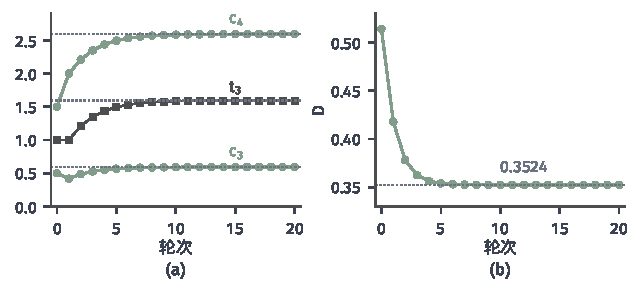
\includegraphics[width=108mm]{figures/07-probability/05-source-coding/matplotlib/quant-lloyd-rounds/figure.pdf}
 \caption{$\operatorname{Laplace}(0,1)$、$N=4$的Lloyd--Max迭代。(a) 正半轴的阈值$t_3$（灰色方块）与重构值$c_3$、$c_4$（绿色圆点）随轮次的变化，点线为不动点。(b) 平均失真随轮次单调下降，点线为不动点处的$0.3524$。}
 \label{fig:quant-lloyd-rounds}
\end{BookInlineFigure}

\paragraph{目标单调下降}
记$D(\mathcal{S},\bm{c})$为区间组$\mathcal{S}$配重构值$\bm{c}$时的平均失真。第$t$轮先由引理~\ref{lem:quant-nearest}，再由引理~\ref{lem:quant-centroid}，得到
\[
 D\bigl(\mathcal{S}^{(t)},\bm{c}^{(t)}\bigr)\leq D\bigl(\mathcal{S}^{(t)},\bm{c}^{(t-1)}\bigr)\leq D\bigl(\mathcal{S}^{(t-1)},\bm{c}^{(t-1)}\bigr) .
\]
所以$D^{(t)}$单调不增。它有下界$0$，因此收敛。

这个论证只说明平均失真的数值收敛，没有说明阈值和重构值本身收敛，更没有说明收敛到最优量化器。例中参数也收敛了，那是这个具体分布的性质。

每轮的代价是计算$N$个区间的概率与一阶矩。分布有显式的积分公式时，代价与$N$成正比；需要数值积分或模拟时，还要加上积分误差，这一点在第~\ref{sec:quant-granular-overload}节再谈。

\paragraph{初始化、空区间与并列}
初始重构值必须互不相同，否则两个点的最近邻区间无法区分。迭代中若某个区间的概率为零，它的条件均值没有定义，式~\eqref{eq:quant-lloyd-update}无法执行。对Laplace这样处处有正密度的读数，只要重构值互不相同，每个区间都有正概率，这种情况不会发生；对离散读数或支撑有空隙的读数则可能发生。常见的处理是保留原来的重构值，或者把它挪到当前误差最大的区间内，把那个区间一分为二。前一种做法仍保证目标不增，后一种改变了迭代的路线，需要重新检查单调性。

读数恰好落在两个重构值的中点时，两者一样近。对有密度的读数，这个事件概率为零；对离散读数，归属约定会改变区间的质心，从而改变后续的迭代，所以必须事先固定，例如一律归入编号较小的区间。

\paragraph{局部最优}
目标下降并不保证到达全局最小。考虑一个离散读数，等概率地取$0$、$2$、$3.5$三个值，用$N=2$个点量化。有两种不同的划分都满足Lloyd--Max条件。

第一种把$\{0\}$与$\{2,3.5\}$分开，重构值是两组的平均：
\[
 c=(0,\ 2.75),\qquad t=1.375 .
\]
$2$离$2.75$比离$0$近，划分与最近邻一致，是不动点。平均失真为
\[
 D=\frac{0+0.75^{2}+0.75^{2}}{3}=0.375 .
\]

第二种把$\{0,2\}$与$\{3.5\}$分开，
\[
 c=(1,\ 3.5),\qquad t=2.25 .
\]
$2$离$1$的距离是$1$，离$3.5$是$1.5$，仍归第一组，也是不动点。平均失真为
\[
 D=\frac{1+1+0}{3}=0.667 .
\]

从$c^{(0)}=(0,1)$出发，阈值$0.5$给出第一种划分；从$c^{(0)}=(1,4)$出发，阈值$2.5$给出第二种划分。两次迭代都在第一轮后停住，结果相差近一倍。图~\ref{fig:quant-lloyd-local}画出这两个不动点。

\begin{BookInlineFigure}
 \centering
 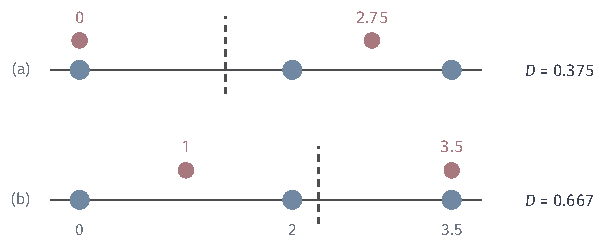
\includegraphics[width=102.5mm]{figures/07-probability/05-source-coding/tikz/quant-lloyd-local/figure.pdf}
 \caption{等概率取$0$、$2$、$3.5$（蓝点）的读数用两个点量化时的两个Lloyd--Max不动点。红点为重构值，虚线为阈值。(a) 划分$\{0\}$、$\{2,3.5\}$，$D=0.375$，是全局最优；(b) 划分$\{0,2\}$、$\{3.5\}$，$D=0.667$，也满足两条必要条件，但不是最优。}
 \label{fig:quant-lloyd-local}
\end{BookInlineFigure}

所以实际计算中常从多组初始值出发，保留平均失真最小的结果。对一维有密度的读数，若密度的对数是凹函数（Laplace与高斯都满足），满足两条条件的量化器只有一个，Lloyd--Max迭代因而收敛到全局最优。证明要说明不动点方程组只有一个解，需要逐个比较阈值的单调性，篇幅较长；上面Laplace例子的不动点方程只有一个正根，与这一结论相符。

\paragraph{与均匀量化的比较}
同样的迭代可以用于任意点数。图~\ref{fig:quant-lloydmax-vs-uniform}比较$N=8$时Lloyd--Max的不动点与最好的均匀量化器（步长在所有$\Delta$中搜索得到）。Lloyd--Max的区间在中央最窄、向外逐渐变宽，最外侧的重构值远达$\pm4.37$；均匀量化器的步长约为$1.03$，范围只到$\pm4.13$。两者的平均失真分别为$0.1090$与$0.1435$，在同样$3$个比特下，按分布调整的划分把误差降低了约$24\%$。

\begin{BookInlineFigure}
 \centering
 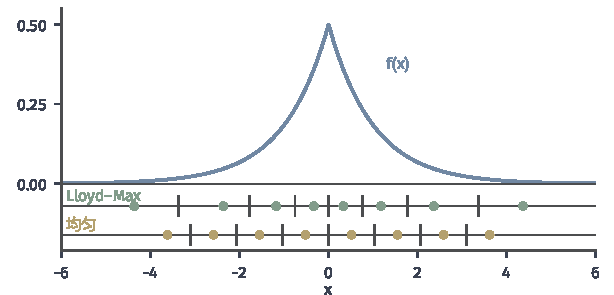
\includegraphics[width=104mm]{figures/07-probability/05-source-coding/matplotlib/quant-lloydmax-vs-uniform/figure.pdf}
 \caption{$\operatorname{Laplace}(0,1)$的两个8点量化器。蓝线为密度。上一行绿点为Lloyd--Max不动点的重构值，竖线为阈值；下一行黄点为最好的均匀量化器的重构值（步长约$1.03$）。Lloyd--Max在中央划得更细、在尾部划得更粗。}
 \label{fig:quant-lloydmax-vs-uniform}
\end{BookInlineFigure}

代价在实现上。均匀量化的编码器按式~\eqref{eq:quant-uniform-encoder}一次除法和取整就能完成，非均匀量化则要把读数与$N-1$个阈值比较（二分查找需要约$\log_2N$次比较），并且需要知道源分布才能设计。


\section{向量量化}
\label{sec:quant-vector}

传感器常常连续读数，相邻两次读数彼此接近。若把每个读数单独量化，量化器看不到这种联系。把两个读数合成一个二维向量，再整体选择重构点，能否在相同的每分量比特数下做得更好？这一节说明答案是肯定的，并说明好处来自哪里、代价在哪里。

\paragraph{逐分量码本与联合码本}
对$d$维读数$\bm{X}=(X_1,\dots,X_d)$，最直接的做法是给每个分量配一个标量量化器，各分量独立编码。若第$i$个分量用$N_i$个点，合起来的重构点是各分量重构值的全部组合，共$N=N_1\cdots N_d$个，区域是坐标轴方向的长方体。这样的量化器称为\term{乘积量化器}（product quantizer），它的码本称为逐分量码本。

更一般的做法是直接在$\mathbb{R}^{d}$中选$N$个点$\bm{c}_1,\dots,\bm{c}_N$作为码本，区域不必是长方体。这就是第~\ref{sec:quant-model}节定义中的$d$维量化器，称为\term{向量量化}（vector quantization），它的码本称为联合码本。乘积量化器是它的特例，所以在相同点数下，最好的联合码本不会比最好的逐分量码本差。按式~\eqref{eq:quant-rate-per-component}，两者每分量的比特数都是$\frac1d\log_2N$。

\paragraph{两条条件的推广}
平方误差取$\lVert\bm{x}-\hat{\bm{x}}\rVert_2^{2}$。第~\ref{sec:quant-nonuniform}节的两个引理在$d$维中照样成立，证明只需把乘积换成内积。

对质心条件，设区域$S$的概率$p>0$，条件均值$\bm{m}=\mathbb{E}[\bm{X}\mid\bm{X}\in S]$。展开平方范数，
\[
 \lVert\bm{X}-\bm{c}\rVert_2^{2}=\lVert\bm{X}-\bm{m}\rVert_2^{2}+2\langle\bm{X}-\bm{m},\bm{m}-\bm{c}\rangle+\lVert\bm{m}-\bm{c}\rVert_2^{2} .
\]
交叉项乘$\mathbf{1}_{\{\bm{X}\in S\}}$后期望为零，于是
\begin{equation}
 \mathbb{E}\bigl[\lVert\bm{X}-\bm{c}\rVert_2^{2}\mathbf{1}_{\{\bm{X}\in S\}}\bigr]=\mathbb{E}\bigl[\lVert\bm{X}-\bm{m}\rVert_2^{2}\mathbf{1}_{\{\bm{X}\in S\}}\bigr]+p\lVert\bm{m}-\bm{c}\rVert_2^{2} ,
 \label{eq:quant-vector-parallel-axis}
\end{equation}
最好的重构点仍是区域的质心。最近邻条件的证明与维数无关，逐点取最近的重构点即可。

最近邻规则下的区域有明确的几何形状。$\bm{x}$离$\bm{c}_j$不比离$\bm{c}_k$远，即
\[
 \lVert\bm{x}-\bm{c}_j\rVert_2^{2}\leq\lVert\bm{x}-\bm{c}_k\rVert_2^{2} .
\]
展开两边，$\lVert\bm{x}\rVert_2^{2}$相消，条件化为
\[
 2\langle\bm{x},\bm{c}_k-\bm{c}_j\rangle\leq\lVert\bm{c}_k\rVert_2^{2}-\lVert\bm{c}_j\rVert_2^{2} .
\]
这是以$\bm{c}_j$与$\bm{c}_k$连线的垂直平分面为边界的半空间。对所有$k\neq j$取交集，得到
\begin{equation}
 V_j=\bigl\{\bm{x}\in\mathbb{R}^{d}:\ \lVert\bm{x}-\bm{c}_j\rVert_2\leq\lVert\bm{x}-\bm{c}_k\rVert_2,\ k=1,\dots,N\bigr\} ,
 \label{eq:quant-voronoi}
\end{equation}
称为$\bm{c}_j$的\term{Voronoi区域}（Voronoi region）。它是有限个半空间的交，因而是凸多面体（可以无界）。各$V_j$只在边界上重叠，边界属于哪一个仍按编号约定；一维时它们就是以中点为端点的区间。

\paragraph{广义Lloyd算法}
于是标量的交替改进可以原样搬过来：固定码本，按式~\eqref{eq:quant-voronoi}把读数分给最近的码字；固定区域，把每个码字移到区域的质心。第~\ref{sec:quant-nonuniform}节的单调性论证逐字适用，平均失真单调不增。这一推广称为\term{广义Lloyd算法}（generalized Lloyd algorithm）。

二维以上的区域是多边形或多面体，质心一般没有显式公式。实际计算时，常用从源分布模拟出的大量向量的平均代替期望：区域的质心换成落在区域中的模拟向量的平均，平均失真换成模拟向量的平均误差。这样得到的是对期望的近似，其误差由第~\ref{chap:monte-carlo-integration-error}章的方法估计；若这些向量不是模拟出来的，而是观测到的数据，从数据估计量化器就属于统计推断的问题，由卷八处理。

\paragraph{相关结构的利用}
先看一个可以手算的例子。读数$\bm{X}=(X_1,X_2)$在两个单位正方形的并集
\[
 A=[0,1]^{2}\cup[1,2]^{2}
\]
上均匀分布，两个正方形各占概率$\tfrac12$。两个分量高度相关：$X_1$小时$X_2$也小。每个分量允许1 bit，即$N=4$。

先用逐分量码本。$X_1$的分布是$[0,1]$与$[1,2]$上各一半的均匀分布，合起来是$[0,2]$上的均匀分布，$X_2$也一样。每个分量最好的两点量化器取区间中点$0.5$与$1.5$，每分量误差为
\[
 \mathbb{E}\bigl[(X_1-Q_1(X_1))^{2}\bigr]=\frac{1^{2}}{12}=\frac{1}{12},
\]
每个向量的平方误差为$\tfrac16$。四个组合点中，$(0.5,1.5)$与$(1.5,0.5)$落在两个空白方块里，它们的区域概率为零，从不被使用。图~\ref{fig:quant-two-squares}左图画出了这种浪费。

\begin{BookInlineFigure}
 \centering
 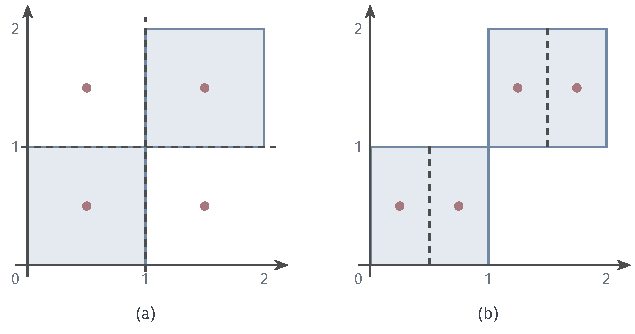
\includegraphics[width=107.5mm]{figures/07-probability/05-source-coding/tikz/quant-two-squares/figure.pdf}
 \caption{在两个单位正方形（浅蓝）上均匀分布的二维读数，用4个点量化。(a) 逐分量码本：每个分量取$0.5$与$1.5$，红点是全部4个组合，虚线是区域边界；两个点落在空白处，从不使用，每个向量的平方误差为$1/6$。(b) 联合码本：每个正方形沿竖直中线一分为二，各放一个质心，平方误差为$5/48$。}
 \label{fig:quant-two-squares}
\end{BookInlineFigure}

若对这个逐分量码本运行广义Lloyd算法，第一轮最近邻分配就会使两个空白方块中的码字分不到任何读数，出现第~\ref{sec:quant-nonuniform}节所说的空区域。按“挪到误差最大的区域并一分为二”的处理，每个被使用的码字区域分出一半给空闲码字，得到右图的联合码本：
\[
 (0.25,0.5),\quad(0.75,0.5),\quad(1.25,1.5),\quad(1.75,1.5) .
\]
每个区域是$\tfrac12\times1$的长方形，读数在其中均匀分布。由式~\eqref{eq:quant-vector-parallel-axis}，以质心为重构点时，误差就是两个坐标方向的方差之和，
\[
 \frac{(1/2)^{2}}{12}+\frac{1^{2}}{12}=\frac{1}{48}+\frac{4}{48}=\frac{5}{48} .
\]
这组码本满足两条条件：每个码字是区域质心，区域也正是最近邻区域。联合码本把每个向量的平方误差从$\tfrac{8}{48}$降到$\tfrac{5}{48}$，减少$37.5\%$，而每分量仍是1 bit。好处来自把四个点全部放在读数真正出现的地方。

图~\ref{fig:quant-gauss-vq}对连续分布做同样的比较。读数是相关系数$0.9$、方差为$1$的二维高斯向量，$N=16$，每分量2 bit。左图是两个4点Lloyd--Max标量量化器的乘积，每分量误差是标量值$0.1175$。十六个长方形中只有十个的概率超过千分之一，其余几乎不用。右图是从左图码本出发、在$2\times10^{5}$个模拟向量上运行广义Lloyd算法得到的联合码本：码字沿对角线排成一串，区域是与对角线垂直的长条。在另外$2\times10^{5}$个独立模拟向量上计算，每分量误差约为$0.0442$，不到逐分量码本的四成。

\begin{BookInlineFigure}
 \centering
 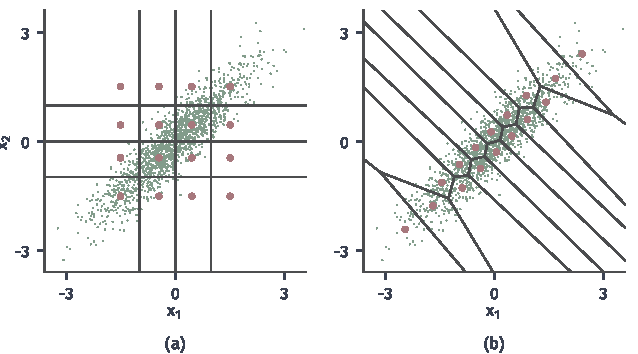
\includegraphics[width=108mm]{figures/07-probability/05-source-coding/matplotlib/quant-gauss-vq/figure.pdf}
 \caption{相关系数$0.9$的二维标准高斯读数，16个码字。绿点为1500个模拟读数，红点为码字，灰线为区域边界。(a) 逐分量4点Lloyd--Max码本，每分量误差$0.1175$。(b) 广义Lloyd算法得到的联合码本（$2\times10^{5}$个训练向量，种子1），区域为Voronoi区域；在独立的$2\times10^{5}$个向量（种子2）上每分量误差约为$0.0442$。}
 \label{fig:quant-gauss-vq}
\end{BookInlineFigure}

\paragraph{区域形状的利用}
即使分量相互独立，联合码本仍有一点好处，来自区域的形状。设读数在一个区域内近似均匀分布，区域面积为$V$，重构点在区域的质心。为了比较形状而不受大小影响，把每分量的平方误差除以$V^{2/d}$，得到无量纲的\term{归一化二阶矩}（normalized second moment）
\begin{equation}
 G=\frac{1}{d}\,\frac{1}{V^{1+2/d}}\int_{\text{区域}}\lVert\bm{x}-\bm{c}\rVert_2^{2}\,\mathrm{d}\bm{x} ,
 \label{eq:quant-normalized-moment}
\end{equation}
$G$越小，同样面积的区域给出的误差越小。逐分量量化在独立同分布的分量上产生正方形区域，联合码本可以用其他形状铺满平面。

单位正方形以中心为重构点时，两个方向各贡献$\tfrac1{12}$，所以$G=\tfrac1{12}\approx0.0833$。正六边形可以用平行轴恒等式~\eqref{eq:quant-vector-parallel-axis}计算。把边长为$a$的正六边形分成六个边长为$a$的正三角形，每个三角形的面积为$A_{\triangle}=\frac{\sqrt3}{4}a^{2}$，直接积分可得它绕自身质心的二阶矩是$A_{\triangle}a^{2}/12$。三角形的质心离六边形中心$a/\sqrt3$，由式~\eqref{eq:quant-vector-parallel-axis}，绕六边形中心的二阶矩为
\[
 A_{\triangle}\Bigl(\frac{a^{2}}{12}+\frac{a^{2}}{3}\Bigr)=\frac{5}{12}A_{\triangle}a^{2} .
\]
六个三角形合起来，面积为$6A_{\triangle}$，二阶矩为$6\cdot\frac{5}{12}A_{\triangle}a^{2}$。取面积为$1$，即$a^{2}=\frac{2}{3\sqrt3}$，代入式~\eqref{eq:quant-normalized-moment}，
\[
 G=\frac12\cdot\frac{5}{12}a^{2}=\frac{5}{36\sqrt3}\approx0.0802 .
\]

\begin{BookInlineFigure}
 \centering
 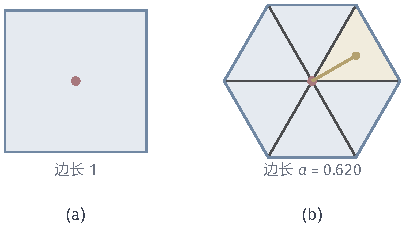
\includegraphics[width=68.6mm]{figures/07-probability/05-source-coding/tikz/quant-cell-shapes/figure.pdf}
 \caption{面积同为$1$的两种区域，红点为重构点。(a) 正方形，$G=1/12\approx0.0833$。(b) 正六边形分成六个正三角形；黄色三角形的质心（黄点）离中心$a/\sqrt3$，由平行轴恒等式求得$G=5/(36\sqrt3)\approx0.0802$。}
 \label{fig:quant-cell-shapes}
\end{BookInlineFigure}

图~\ref{fig:quant-cell-shapes}比较了这两种形状。六边形比正方形更接近圆，离重构点远的角少，在相同面积下误差约小$3.8\%$。这个收益只在区域很多、边界效应可以忽略时才显现，而且只有联合码本才能取得，因为逐分量量化的区域永远是长方体。与相关结构带来的收益相比，形状收益不大；但它说明即使分量独立，逐个读数量化也不是最好的做法。

\paragraph{存储、搜索与局部最优的代价}
联合码本的收益需要付出代价。固定每分量$R$个比特，码字个数为
\begin{equation}
 N=2^{dR} ,
 \label{eq:quant-codebook-size}
\end{equation}
随维数$d$指数增长。表~\ref{tab:quant-vq-cost}列出几种情形：存储码本需要$Nd$个实数，对每个读数做穷举最近邻搜索需要计算$N$个距离，约$Nd$次乘法。逐分量码本只需存储$d$个标量量化器，共$d2^{R}$个数，编码时各分量独立查找。

\begin{BookInlineTable}
 \centering
 \begin{tabular}{rrrrr}
  \toprule
  $d$ & $R$ & $N=2^{dR}$ & 联合码本存储$Nd$ & 逐分量存储$d2^{R}$\\
  \midrule
  $2$ & $2$ & $16$ & $32$ & $8$\\
  $4$ & $2$ & $256$ & $1024$ & $16$\\
  $8$ & $2$ & $65536$ & $524288$ & $32$\\
  $16$ & $1$ & $65536$ & $1048576$ & $32$\\
  \bottomrule
 \end{tabular}
 \caption{每分量$R$ bit时联合码本与逐分量码本的规模。穷举搜索每个读数的乘法次数与联合码本存储量同阶。}
 \label{tab:quant-vq-cost}
\end{BookInlineTable}

设计码本也更困难。广义Lloyd算法每轮要对每个模拟向量计算$N$个距离，而且目标函数有许多局部最小值，结果依赖初值。图~\ref{fig:quant-vq-inits}在前面的相关高斯例子上，从十组随机初值出发各迭代四十轮：所有轨迹都降到逐分量码本的误差之下，最终的每分量误差分布在$0.0439$到$0.0455$之间，彼此相差约$4\%$。维数和码字更多时，这种差异通常更大。

\begin{BookInlineFigure}
 \centering
 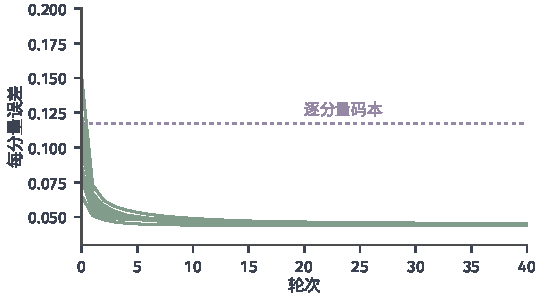
\includegraphics[width=92mm]{figures/07-probability/05-source-coding/matplotlib/quant-vq-inits/figure.pdf}
 \caption{相关系数$0.9$的二维高斯读数、16个码字时，广义Lloyd算法从十组初值出发的每分量误差（绿线，在$5\times10^{4}$个模拟向量上计算，种子1；初值为随机抽取的16个模拟向量，种子11至20）。紫色点线为逐分量4点Lloyd--Max码本的误差$0.1175$。各轨迹单调下降，但停在不同的值上。}
 \label{fig:quant-vq-inits}
\end{BookInlineFigure}

所以向量量化的维数是一种权衡：维数越高，越能利用相关结构和区域形状，码本存储、搜索和设计的代价也越高。实际系统常用有结构的码本（例如由格点构成的码本，或分级、分组的码本）来降低搜索代价，代价是放弃一部分失真上的收益。


\section{量化索引的压缩}
\label{sec:quant-index-coding}

到目前为止，每个索引都按定长写出，$N$个点用$\log_2N$个比特。可是索引并不等可能：Laplace读数的四点Lloyd--Max量化器中，内侧两个区间各占约$40\%$，外侧两个各占约$10\%$。上一章说过，概率不均匀的离散信源可以用变长码缩短平均长度。量化索引正是这样一个离散信源。

\paragraph{固定量化器后的索引编码}
量化器固定后，索引$J=\alpha(X)$的分布由式~\eqref{eq:quant-index-pmf}给出。对$J$使用第~\ref{chap:lossless-coding}章的前缀码，接收端能精确恢复$J$，再由解码器报出同一个重构值。重构结果、从而平均失真都没有改变，改变的只是平均描述长度。由上一章的平均码长界，最好的前缀码满足
\begin{equation}
 H(J)\leq\bar{\ell}<H(J)+1 ,
 \label{eq:quant-index-length-bound}
\end{equation}
其中$\bar{\ell}=\sum_jp_j\ell(j)$是平均码长，$H(J)$是索引的熵。

以第~\ref{sec:quant-nonuniform}节得到的四点不动点量化器为例。外侧区间$\lvert X\rvert\geq1.5936$的概率是$\mathrm{e}^{-1.5936}=0.2032$，两侧平分，于是索引的分布为
\[
 (p_1,p_2,p_3,p_4)=(0.1016,\ 0.3984,\ 0.3984,\ 0.1016) .
\]
它的熵为
\[
 H(J)=-2\bigl(0.1016\log_20.1016+0.3984\log_20.3984\bigr)=1.728\ \text{bit} .
\]

用Huffman编码构造码树：先合并两个最小的概率$0.1016$与$0.1016$，得$0.2032$；再与一个$0.3984$合并，得$0.6016$；最后与另一个$0.3984$合并。码长依次为$1,2,3,3$，平均码长为
\[
 \bar{\ell}=0.3984\times1+0.3984\times2+0.1016\times3\times2=1.805\ \text{bit} .
\]
图~\ref{fig:quant-index-huffman}画出了这棵码树。与定长的$2$个比特相比，平均每个读数省下约$0.2$个比特，平均失真仍是$0.3524$。若把两个读数的索引组成一对再编码，每读数的平均码长不超过$H(J)+\tfrac12$；块越长，越接近$1.728$。

\begin{BookInlineFigure}
 \centering
 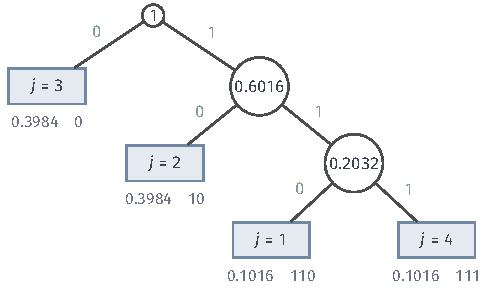
\includegraphics[width=83.4mm]{figures/07-probability/05-source-coding/tikz/quant-index-huffman/figure.pdf}
 \caption{$\operatorname{Laplace}(0,1)$四点Lloyd--Max量化器索引的Huffman码树。叶结点下方是区间概率与码字，内部结点标出合并后的概率，绿色数字是分支标号。平均码长为$1.805$ bit，索引的熵为$1.728$ bit。}
 \label{fig:quant-index-huffman}
\end{BookInlineFigure}

\paragraph{均匀量化配合熵编码}
变长描述还改变了对有限范围的要求。定长索引必须事先限定点数，因而必须规定表示范围，范围外的读数产生过载误差。变长描述却可以使用无穷多个区间：取步长为$\Delta$、零为重构值的均匀刻度，
\begin{equation}
 Q_{\Delta}(x)=\Delta\Bigl\lfloor\frac{x}{\Delta}+\frac12\Bigr\rfloor ,
 \label{eq:quant-midtread}
\end{equation}
它把$[(k-\frac12)\Delta,(k+\frac12)\Delta)$映到$k\Delta$，$k$取遍全体整数。远处的区间概率极小，给它们很长的码字，对平均长度几乎没有影响，而误差始终不超过$\Delta/2$。

索引集合可数无穷时，Huffman编码的构造不再直接适用，但长度为$\ell(k)=\lceil-\log_2p_k\rceil$的前缀码仍然存在：这些长度满足$\sum_k2^{-\ell(k)}\leq\sum_kp_k=1$，按长度从短到长依次在码树上分配码字即可，平均长度小于$H(J)+1$。所以对均匀量化配合熵编码，描述资源由索引的熵衡量。

\paragraph{索引熵与微分熵}
步长很小时，索引的熵可以用读数的微分熵近似。回顾第~\ref{chap:information-measures}章，具有密度$f$的读数的微分熵是
\[
 h(X)=-\int f(x)\log_2f(x)\,\mathrm{d}x .
\]
对Laplace读数，$-\log_2f(x)=1+\lvert x\rvert\log_2\mathrm{e}$，又$\mathbb{E}\lvert X\rvert=1$，所以
\[
 h(X)=1+\log_2\mathrm{e}=\log_2(2\mathrm{e})\approx2.443\ \text{bit} .
\]

若密度在每个长度为$\Delta$的区间内变化不大，区间概率近似为$p_k\approx f(k\Delta)\Delta$。代入索引的熵，
\[
 H(J)=-\sum_kp_k\log_2p_k\approx-\sum_kp_k\log_2f(k\Delta)-\log_2\Delta .
\]
第一项是$-\log_2f$在区间代表点上按区间概率加权的和，在$\Delta\to0$时趋于积分$h(X)$。于是
\begin{equation}
 H\bigl(Q_{\Delta}(X)\bigr)\approx h(X)-\log_2\Delta .
 \label{eq:quant-index-entropy-highres}
\end{equation}
步长减半，索引的熵增加一个比特，相当于每个区间分成两半、需要多问一个是非题。在密度足够规则（例如Riemann可积且$H(Q_1(X))$有限）时，式~\eqref{eq:quant-index-entropy-highres}两边之差在$\Delta\to0$时趋于零，证明可查阅~\scite{math-cover2006information}。

\begin{BookInlineFigure}
 \centering
 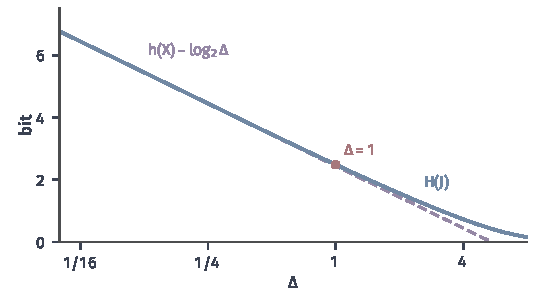
\includegraphics[width=92mm]{figures/07-probability/05-source-coding/matplotlib/quant-entropy-step/figure.pdf}
 \caption{$\operatorname{Laplace}(0,1)$读数经步长为$\Delta$的无穷均匀量化器~\eqref{eq:quant-midtread}后索引的熵。蓝线为精确值，紫色虚线为近似$h(X)-\log_2\Delta$，$h(X)=\log_2(2\mathrm{e})$；横轴为对数刻度。红点为$\Delta=1$，精确值$2.484$ bit，近似值$2.443$ bit。}
 \label{fig:quant-index-entropy}
\end{BookInlineFigure}

图~\ref{fig:quant-index-entropy}比较两者。$\Delta=1$时精确值为$2.484$ bit，近似值为$2.443$ bit，已经相当接近；步长再小，两条曲线几乎重合。步长大到与分布的尺度相当时近似失效：$\Delta=4$时近似值为负，而熵不可能为负，此时中央区间的概率已达$0.865$。

\paragraph{比较时固定相同的资源}
现在可以在相同的平均描述长度下比较不同方案。图~\ref{fig:quant-operational}画出Laplace读数的平均失真随每读数比特数的变化。黄线和绿线是定长索引的最好均匀量化器与Lloyd--Max量化器，横坐标为$\log_2N$；蓝线是无穷均匀量化器配合熵编码，横坐标为索引的熵$H(J)$；红点是四点Lloyd--Max量化器配合熵编码。

\begin{BookInlineFigure}
 \centering
 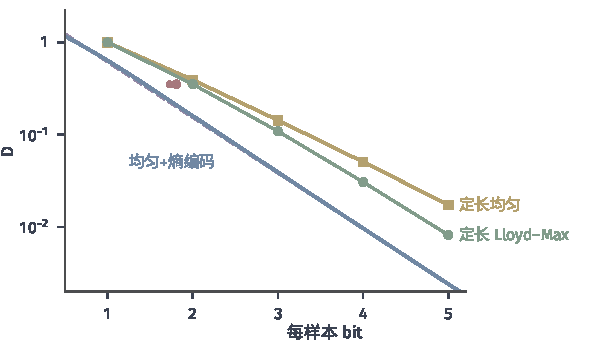
\includegraphics[width=100mm]{figures/07-probability/05-source-coding/matplotlib/quant-operational/figure.pdf}
 \caption{$\operatorname{Laplace}(0,1)$读数的平均失真与每读数比特数（纵轴为对数刻度）。黄色方块：定长索引的最好均匀量化器，$N=2,4,\dots,32$；绿色圆点：定长索引的Lloyd--Max量化器；蓝线：无穷均匀量化器配合熵编码，横坐标为索引的熵；紫色虚线：高分辨率公式$\frac{(2\mathrm{e})^{2}}{12}2^{-2R}$，与蓝线几乎重合；红点：四点Lloyd--Max量化器配合Huffman码（$1.805$ bit）与理想码长（$1.728$ bit）。}
 \label{fig:quant-operational}
\end{BookInlineFigure}

图中的排序很清楚。在约$1.8$ bit处，四点Lloyd--Max量化器加Huffman码的失真是$0.352$，而步长约为$1.66$的均匀量化器加熵编码，失真只有$0.212$。在定长$3$ bit处，Lloyd--Max量化器的失真是$0.109$；均匀量化器加熵编码只用约$2.5$ bit（$\Delta=1$）就达到$0.081$。分布越不均匀、尾部越重，这种差距越明显。

蓝线在比特数较大时几乎是一条直线，斜率对应“每多一个比特，失真降为四分之一”。这可以由两个近似合起来解释：范围内的误差近似为$\Delta^{2}/12$（第~\ref{sec:quant-granular-overload}节），索引熵近似为式~\eqref{eq:quant-index-entropy-highres}。消去$\Delta$，得到平均描述长度为$R$时
\begin{equation}
 D\approx\frac{1}{12}\,2^{2h(X)}\,2^{-2R} .
 \label{eq:quant-highres-ec}
\end{equation}
这是一个高分辨率近似，紫色虚线就是它；在$R$较小时它不再可靠。

\paragraph{把码长写进目标}
上面的方案先设计量化器、再压缩索引，两步是分开的。若平均码长才是真正的预算，那么区间和重构值也应当按这个预算来设计，而不是按点数来设计。这时“固定点数$N$”不再代表固定的描述资源：一个有许多点、但大部分点概率很小的量化器，平均码长可以很短。

把平均码长写进目标，对给定的乘子$\lambda>0$，最小化
\begin{equation}
 J_{\lambda}=D+\lambda\bar{\ell}=\mathbb{E}\bigl[(X-c_{\alpha(X)})^{2}\bigr]+\lambda\,\mathbb{E}\bigl[\ell(\alpha(X))\bigr] .
 \label{eq:quant-ecsq-objective}
\end{equation}
$\lambda$表示一个比特值多少平方误差：$\lambda$大，就更看重短码。改变$\lambda$得到不同的失真与码长组合。这样设计的量化器称为\term{熵约束量化}（entropy-constrained quantization）。

式~\eqref{eq:quant-ecsq-objective}仍是逐点代价的期望，读数$x$归入区间$j$的代价是$(x-c_j)^{2}+\lambda\ell(j)$。所以最近邻条件要修改为：把读数分给使这个带罚代价最小的$j$。比较相邻的两个重构值$c_j<c_{j+1}$，读数归入$j$当且仅当
\[
 (x-c_j)^{2}+\lambda\ell(j)\leq(x-c_{j+1})^{2}+\lambda\ell(j+1) .
\]
展开后，与第~\ref{sec:quant-nonuniform}节的计算相同，阈值从中点移到
\begin{equation}
 t_j=\frac{c_j+c_{j+1}}{2}+\frac{\lambda\bigl(\ell(j+1)-\ell(j)\bigr)}{2(c_{j+1}-c_j)} .
 \label{eq:quant-ecsq-threshold}
\end{equation}
码长较长的那个重构值，区间被压缩；读数要离它足够近，节省的误差才抵得上多付的码长。

以四点Lloyd--Max量化器为起点，取理想码长$\ell(j)=-\log_2p_j$，即内侧$1.328$ bit、外侧$3.299$ bit，以及$\lambda=0.5$。由式~\eqref{eq:quant-ecsq-threshold}，正半轴的阈值从$1.5936$移到
\[
 t_3=1.5936+\frac{0.5\times(3.299-1.328)}{2\times2}=1.840 .
\]
图~\ref{fig:quant-ecsq-threshold}画出了带罚代价的两条抛物线和移动后的交点。

\begin{BookInlineFigure}
 \centering
 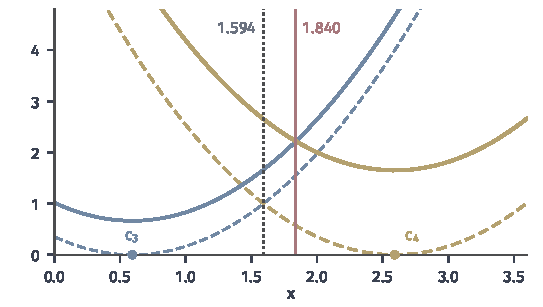
\includegraphics[width=92mm]{figures/07-probability/05-source-coding/matplotlib/quant-ecsq-threshold/figure.pdf}
 \caption{熵约束下的阈值。蓝色与黄色分别对应内侧重构值$c_3=0.594$（码长$1.328$ bit）与外侧重构值$c_4=2.594$（码长$3.299$ bit）。虚线为$(x-c_j)^{2}$，交于中点$1.594$；实线为$(x-c_j)^{2}+\lambda\ell(j)$，$\lambda=0.5$，交点右移到$1.840$（红线）。}
 \label{fig:quant-ecsq-threshold}
\end{BookInlineFigure}

阈值确定后，接着做两件事：把重构值移到新区间的质心，再把码长更新为新区间概率的理想码长。例中外侧区间概率降为$\mathrm{e}^{-1.840}/2=0.0794$，内侧升为$0.4206$；由式~\eqref{eq:quant-laplace-centroid}，新的质心为
\[
 c_3=0.6526,\qquad c_4=2.8400 .
\]
新的码长为$1.250$ bit与$3.655$ bit。平均失真升到$0.3608$，平均码长降到$1.631$ bit，目标$J_{0.5}$从$0.3524+0.5\times1.728=1.2165$降到$1.1765$。

这三步各自不增加$J_{\lambda}$。分配一步是对每个读数取带罚代价最小的区间，质心一步只改变失真项，理由与第~\ref{sec:quant-nonuniform}节相同。码长一步固定区间概率$p_j$，在$\sum_j2^{-\ell(j)}\leq1$下最小化$\sum_jp_j\ell(j)$；允许非整数码长时，上一章用KL散度的非负性证明了最小值在$\ell(j)=-\log_2p_j$取到，等于$H(J)$。实际码长必须是整数，理想码长只是这一步的近似，实际平均码长比它多不到一个比特，用块编码可以把这部分摊薄。

$\lambda$越大，外侧区间越被压缩，最终某些区间的概率可能趋于零，相当于自动减少了点数。在高分辨率下，可以说明熵约束量化的最优解接近均匀刻度，这与图~\ref{fig:quant-operational}中均匀量化加熵编码表现最好是一致的。总之，固定点数与固定平均码率是两种不同的约束，以平均码长为预算时，必须把它写进设计目标。


\section{量化误差}
\label{sec:quant-error}

前几节只用平均失真一个数评价量化器。误差本身是一个随机变量，记为
\[
 E=Q(X)-X .
\]
关于它还可以问三个问题：典型的大小是多少，偶尔会大到什么程度，它与读数之间有什么关系。第一个问题决定平均失真，第二个问题关系到最坏情形，第三个问题关系到能否把量化看成“读数加上一点独立噪声”。这一节对已经构造的量化器回答这三个问题，并说明加入共享的随机扰动怎样改变第三个问题的答案。

\subsection{舍入误差与过载误差}
\label{sec:quant-granular-overload}

考虑第~\ref{sec:quant-uniform}节的均匀量化器：$N$个点、步长$\Delta$、范围$[-L,L]$，$L=N\Delta/2$，范围外饱和。按读数是否落在范围内，把平均失真分成两部分：
\begin{equation}
 D=\underbrace{\mathbb{E}\bigl[E^{2}\mathbf{1}_{\{\lvert X\rvert\leq L\}}\bigr]}_{D_{\mathrm{gran}}}+\underbrace{\mathbb{E}\bigl[E^{2}\mathbf{1}_{\{\lvert X\rvert>L\}}\bigr]}_{D_{\mathrm{over}}} .
 \label{eq:quant-granular-overload}
\end{equation}
第一部分是舍入误差的贡献，第二部分是过载误差的贡献。

\paragraph{误差随读数的变化}
图~\ref{fig:quant-error-shape}左图画出$N=8$、$\Delta=1$时误差随读数的变化。范围内误差是锯齿形，在每个区间内从$+\tfrac12$线性降到$-\tfrac12$；范围外误差随读数线性增长，没有上界。

\begin{BookInlineFigure}
 \centering
 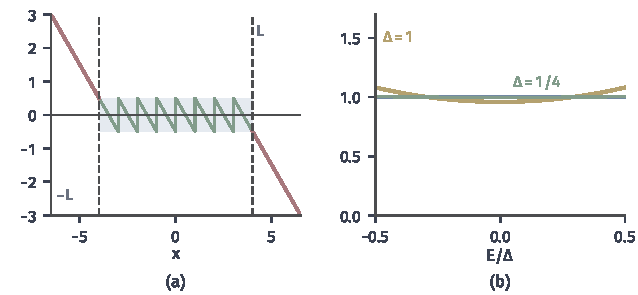
\includegraphics[width=108mm]{figures/07-probability/05-source-coding/matplotlib/quant-error-shape/figure.pdf}
 \caption{均匀量化的误差。(a) $N=8$、$\Delta=1$时$E=Q(x)-x$随读数的变化：范围内（浅蓝带，$\lvert E\rvert\leq\frac12$）为绿色锯齿，范围外为红色直线。(b) 对$\operatorname{Laplace}(0,1)$读数，在不过载的条件下$E/\Delta$的精确密度：黄线为$\Delta=1$（$N=8$），绿线为$\Delta=1/4$（$N=32$），两者范围同为$[-4,4]$；蓝线为均匀密度$1$。}
 \label{fig:quant-error-shape}
\end{BookInlineFigure}

\paragraph{舍入误差}
范围内的读数与所在区间的中点相距不超过$\Delta/2$，所以总有
\[
 D_{\mathrm{gran}}\leq\frac{\Delta^{2}}{4}\,\mathbb{P}\bigl(\lvert X\rvert\leq L\bigr) .
\]
这个界对任何分布都成立，但通常偏大四倍左右。

更常用的是一个近似。若密度在每个区间内几乎不变，那么在读数落在某个区间的条件下，它近似均匀分布于这个区间，误差近似均匀分布于$[-\Delta/2,\Delta/2]$。对均匀分布直接积分，
\[
 \frac{1}{\Delta}\int_{-\Delta/2}^{\Delta/2}e^{2}\,\mathrm{d}e=\frac{\Delta^{2}}{12} .
\]
把各区间合起来，得到
\begin{equation}
 D_{\mathrm{gran}}\approx\frac{\Delta^{2}}{12}\,\mathbb{P}\bigl(\lvert X\rvert\leq L\bigr) .
 \label{eq:quant-granular-approx}
\end{equation}
这称为\term{高分辨率近似}（high-resolution approximation）。它不是精确公式：条件是密度在区间尺度上变化很小，$\Delta$越小越准确。

近似的偏差可以用质心条件看清楚。由引理~\ref{lem:quant-centroid}，一个区间内以中点$c_j$为重构值的条件平方误差，等于条件方差加上质心与中点距离的平方。以Laplace读数的区间$[0,1)$为例，在$0\leq X<1$的条件下，由式~\eqref{eq:quant-laplace-centroid}与二阶矩的积分，得到
\[
 \operatorname{Var}(X\mid0\leq X<1)=0.0793,\qquad (0.5-0.4180)^{2}=0.0067 .
\]
二者相加为$0.0860$，而均匀近似给出$\tfrac1{12}=0.0833$。条件方差比$\tfrac1{12}$小，因为质量偏向区间左端；但重构值不在质心，又多出一项。图~\ref{fig:quant-error-shape}右图画出了合起来的效果：$\Delta=1$时误差的密度在$0.96$到$1.08$之间起伏，$\Delta=1/4$时已几乎是常数$1$。

非均匀量化器的区间长度$\Delta_j$各不相同，式~\eqref{eq:quant-granular-approx}相应地改为
\[
 D_{\mathrm{gran}}\approx\sum_{j}\frac{p_j\Delta_j^{2}}{12} .
\]
概率$p_j$大的区间若取得窄，就能减小这个和；这正是Lloyd--Max量化器在中央划得细的原因。

\paragraph{过载误差}
对Laplace读数，过载部分有显式公式。看右侧：读数$X>L$时报出$c_N=L-\Delta/2$，误差的绝对值是$(X-L)+\Delta/2$。在$X>L$的条件下，超出量$X-L$服从$\operatorname{Exp}(1)$，记为$Z$。对$a=\Delta/2$，
\[
 \mathbb{E}\bigl[(Z+a)^{2}\bigr]=\mathbb{E}[Z^{2}]+2a\,\mathbb{E}[Z]+a^{2}=2+2a+a^{2} .
\]
右侧过载的概率是$\mathrm{e}^{-L}/2$，左右对称，于是
\begin{equation}
 D_{\mathrm{over}}=\mathrm{e}^{-L}\Bigl(\frac{\Delta^{2}}{4}+\Delta+2\Bigr),\qquad L=\frac{N\Delta}{2} .
 \label{eq:quant-laplace-overload}
\end{equation}
它随$L$指数衰减。尾部越轻，过载误差衰减越快；尾部更重的分布，例如按幂律衰减的分布，需要更大的范围才能把过载压下去。

\paragraph{步长的权衡}
把$N=8$代入，$L=4\Delta$。由式~\eqref{eq:quant-granular-approx}与式~\eqref{eq:quant-laplace-overload}，
\[
 D(\Delta)\approx\frac{\Delta^{2}}{12}\bigl(1-\mathrm{e}^{-4\Delta}\bigr)+\mathrm{e}^{-4\Delta}\Bigl(\frac{\Delta^{2}}{4}+\Delta+2\Bigr) .
\]
下面算三个步长。$\Delta=0.5$时范围只到$\pm2$，过载占主导：
\[
 D_{\mathrm{gran}}\approx0.0180,\qquad D_{\mathrm{over}}=0.3468 .
\]
$\Delta=1$时两者相当：
\[
 D_{\mathrm{gran}}\approx0.0818,\qquad D_{\mathrm{over}}=0.0595 .
\]
$\Delta=1.5$时范围到$\pm6$，过载几乎消失，舍入占主导：
\[
 D_{\mathrm{gran}}\approx0.1870,\qquad D_{\mathrm{over}}=0.0101 .
\]
三者的总和约为$0.365$、$0.141$和$0.197$。舍入部分的精确值分别为$0.0182$、$0.0845$与$0.2004$，均匀近似在$\Delta=1.5$时偏小约$7\%$。

图~\ref{fig:quant-gran-overload}画出两部分随步长的完整变化。总误差在$\Delta^{*}\approx1.03$处最小，最小值为$0.1435$，此时舍入部分约占$63\%$。在最优点附近，两部分的变化率相互抵消：再缩小步长，过载的增加超过舍入的减少。

\begin{BookInlineFigure}
 \centering
 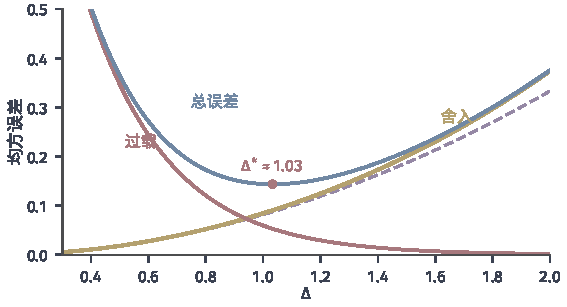
\includegraphics[width=96mm]{figures/07-probability/05-source-coding/matplotlib/quant-gran-overload/figure.pdf}
 \caption{$\operatorname{Laplace}(0,1)$读数、$N=8$的均匀量化器的平均失真随步长的变化，范围$L=4\Delta$。黄线为舍入部分的精确值，紫色虚线为其近似$\frac{\Delta^2}{12}\mathbb{P}(\lvert X\rvert\leq L)$，红线为过载部分~\eqref{eq:quant-laplace-overload}，蓝线为总和；红点为最优步长$\Delta^{*}\approx1.03$。}
 \label{fig:quant-gran-overload}
\end{BookInlineFigure}

\paragraph{点数的权衡}
增加点数时，最优步长与范围一起变化。表~\ref{tab:quant-uniform-points}列出对每个$N$搜索最优步长的结果。点数每加倍，最优范围大约增加$1.1$，而不是保持不变：为了让过载项$\mathrm{e}^{-L}$与舍入项$\Delta^{2}/12$同步减小，范围必须随点数缓慢变宽。所以步长缩小不到一半，每多一个比特，失真只降为原来的$0.35$左右，而不是理想的四分之一。

\begin{BookInlineTable}
 \centering
 \begin{tabular}{rrrrrr}
  \toprule
  $N$ & $\Delta^{*}$ & $L^{*}$ & 舍入 & 过载 & 总失真\\
  \midrule
  $4$ & $1.538$ & $3.08$ & $0.2020$ & $0.1906$ & $0.3926$\\
  $8$ & $1.034$ & $4.13$ & $0.0907$ & $0.0528$ & $0.1435$\\
  $16$ & $0.652$ & $5.22$ & $0.0357$ & $0.0150$ & $0.0507$\\
  $32$ & $0.396$ & $6.34$ & $0.0131$ & $0.0043$ & $0.0174$\\
  \bottomrule
 \end{tabular}
 \caption{$\operatorname{Laplace}(0,1)$读数的最优均匀量化器（定长索引）。舍入与过载为精确值；同样点数的Lloyd--Max量化器失真依次为$0.3524$、$0.1090$、$0.0307$、$0.0082$。}
 \label{tab:quant-uniform-points}
\end{BookInlineTable}

\paragraph{误差的尾部}
平均失真之外，有时还关心误差偶尔有多大。范围内的误差总不超过$\Delta/2$，超过$\Delta/2$的误差只能来自过载。对$s\geq\Delta/2$，$\lvert E\rvert>s$等价于$\lvert X\rvert>L-\Delta/2+s$，所以
\[
 \mathbb{P}\bigl(\lvert E\rvert>s\bigr)=\mathrm{e}^{-(L-\Delta/2+s)},\qquad s\geq\frac{\Delta}{2} .
\]
$N=8$、$\Delta=1$时，误差超过$0.5$的概率是$\mathrm{e}^{-4}=0.018$，超过$1$的概率是$\mathrm{e}^{-4.5}=0.011$，超过$2$的概率是$\mathrm{e}^{-5.5}=0.004$。误差没有上界，但它的尾部继承了读数的尾部。需要保证最坏误差时，只能加大范围或另外描述越界的读数。

\paragraph{误差与读数的关系}
误差$E=Q(X)-X$是读数的函数，给定读数，误差就完全确定。所以$E$与$X$不可能独立（除非$E$几乎必然为常数）。即使只看相关性，误差与读数一般也相关：若重构值都是质心，由第~\ref{sec:quant-nonuniform}节的正交性，$\mathbb{E}[EQ(X)]=0$，而$X=Q(X)-E$，于是
\[
 \mathbb{E}[XE]=\mathbb{E}[Q(X)E]-\mathbb{E}[E^{2}]=-D .
\]
又$\mathbb{E}[E]=0$，所以$\operatorname{Cov}(X,E)=-D\neq0$。

常用的“加性噪声模型”把量化写成$Q(X)=X+E$，并假定$E$与$X$独立、在$[-\Delta/2,\Delta/2]$上均匀分布。上面的讨论说明这只是一个近似：在高分辨率下，误差的分布接近均匀（图~\ref{fig:quant-error-shape}右图），与读数的相关系数$-\sqrt{D}/\sqrt{\operatorname{Var}(X)}$趋于零，用它估算平均失真是合理的；但在粗量化、有过载，或读数本身取值规则（例如总落在刻度附近、长时间停在同一个区间内）时，它会给出错误的结论。第~\ref{sec:quant-dither}节给出一种使这个模型精确成立的办法。

\paragraph{期望难以计算时}
上面的平均失真都由显式积分得到。分布或区域复杂时，例如向量量化的Voronoi区域，期望难以直接积分，可以用模拟的平均代替：独立地生成$n$个读数，计算误差平方的样本平均。它本身是期望的一个估计，有自己的随机误差，应当与量化误差分开报告。例如对$N=8$、$\Delta=1$的Laplace例子，用$n=10^{5}$个模拟读数（种子7），得到估计$0.1438$，标准误差约$0.0025$；精确值$0.1440$在其范围之内。模拟误差怎样随$n$缩小、怎样给出可靠的区间，见第~\ref{chap:monte-carlo-integration-error}章。

\paragraph{比较的前提}
比较两个量化器时，源分布、失真函数和描述资源必须相同。表~\ref{tab:quant-uniform-points}与图~\ref{fig:quant-operational}都遵守这一点：同一个Laplace读数、平方误差，横向比较时固定点数或固定平均码长。单纯增加点数总能降低误差，但同时增加存储、搜索与描述长度；说一个量化器“更好”，必须说明是在哪种资源下更好。

\subsection{抖动对误差的影响}
\label{sec:quant-dither}

确定性量化的误差由读数决定，这在某些场合是个实际问题。设读数长时间停在$x=0.3$附近，用步长$\Delta=1$、零为重构值的无穷均匀量化器~\eqref{eq:quant-midtread}，每次都报$0$，误差恒为$-0.3$。多次记录再平均也消除不了这个偏差，因为误差没有任何随机性可以被平均掉。能否让误差变成与读数无关的随机量？

\paragraph{减性抖动}
办法是在量化前给读数加一个随机扰动，并让解码器知道同一个扰动，重构时再把它减掉。设$U$与$X$独立，服从$[-\Delta/2,\Delta/2)$上的均匀分布。编码器量化$X+U$，传送索引；解码器取得同一个$U$的值（例如双方使用同一个伪随机数发生器和种子），输出
\begin{equation}
 \hat{X}=Q_{\Delta}(X+U)-U .
 \label{eq:quant-subtractive-dither}
\end{equation}
这称为\term{减性抖动}（subtractive dither），所加的扰动称为\term{抖动}（dither）。重构误差为
\[
 E=\hat{X}-X=Q_{\Delta}(X+U)-(X+U) ,
\]
也就是对$V=X+U$做舍入的误差。

先用$x=0.3$、$\Delta=1$手算三个扰动值。取$u=0.37$，$v=0.67$舍入到$1$，于是
\[
 \hat{x}=1-0.37=0.63,\qquad E=0.33 .
\]
取$u=-0.42$，$v=-0.12$舍入到$0$，于是
\[
 \hat{x}=0+0.42=0.42,\qquad E=0.12 .
\]
取$u=0.1$，$v=0.4$舍入到$0$，于是
\[
 \hat{x}=-0.1,\qquad E=-0.4 .
\]
同一个读数，误差随扰动变化，有正有负。

\paragraph{误差的分布}
为什么误差会均匀？固定$x$，$V=x+U$均匀分布在一个长度恰为$\Delta$的区间$[x-\Delta/2,x+\Delta/2)$上。这个区间恰好跨过一个刻度区间的边界，把它切成两段：左段舍入到一个刻度，右段舍入到下一个刻度。两段上的舍入误差$Q_{\Delta}(v)-v$各自扫过$[-\Delta/2,\Delta/2)$的一部分，拼起来恰好扫过一遍。图~\ref{fig:quant-dither-mechanism}画出$x=0.3$的情形。

\begin{BookInlineFigure}
 \centering
 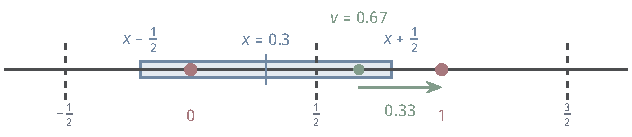
\includegraphics[width=107.1mm]{figures/07-probability/05-source-coding/tikz/quant-dither-mechanism/figure.pdf}
 \caption{减性抖动的机制，$\Delta=1$，$x=0.3$。浅蓝带是$V=x+U$的取值范围$[-0.2,0.8)$，红点是刻度$0$与$1$，虚线是区间边界。带中$[-0.2,0.5)$部分舍入到$0$，误差$-v$取遍$(-0.5,0.2]$；$[0.5,0.8)$部分舍入到$1$，误差$1-v$取遍$(0.2,0.5]$。绿点为$u=0.37$时的$v=0.67$，箭头长度是误差$0.33$。}
 \label{fig:quant-dither-mechanism}
\end{BookInlineFigure}

\begin{theorem}[减性抖动的误差]
\label{thm:quant-subtractive-dither}
设$Q_{\Delta}$为式~\eqref{eq:quant-midtread}的无穷均匀量化器，$U$服从$[-\Delta/2,\Delta/2)$上的均匀分布且与$X$独立。则式~\eqref{eq:quant-subtractive-dither}的重构误差$E=\hat{X}-X$服从$(-\Delta/2,\Delta/2]$上的均匀分布，并且与$X$独立。特别地，
\begin{equation}
 \mathbb{E}[E]=0,\qquad \mathbb{E}[E^{2}]=\frac{\Delta^{2}}{12} ,
 \label{eq:quant-dither-moments}
\end{equation}
对任何读数分布成立。
\end{theorem}

\begin{proof}
记$g(v)=Q_{\Delta}(v)-v$，它是周期为$\Delta$的函数，在$[k\Delta-\Delta/2,k\Delta+\Delta/2)$上等于$k\Delta-v$，取值于$(-\Delta/2,\Delta/2]$。于是$E=g(X+U)$。

先固定$x$，计算$g(x+U)$的分布。$x+U$在$I_x=[x-\Delta/2,x+\Delta/2)$上均匀分布，密度为$1/\Delta$。对$(-\Delta/2,\Delta/2]$中的Borel集$B$，
\[
 \mathbb{P}\bigl(g(x+U)\in B\bigr)=\frac{1}{\Delta}\,\lambda\bigl(\{v\in I_x:g(v)\in B\}\bigr) ,
\]
$\lambda$为长度。$I_x$长度恰为$\Delta$，按刻度区间的边界把它切成至多两段，每段上$g(v)=k\Delta-v$是斜率为$-1$的平移，保持长度。两段的像拼起来恰为$(-\Delta/2,\Delta/2]$，互不重叠，因为$g$的周期为$\Delta$，长度为$\Delta$的区间上每个误差值恰好出现一次。所以上式右边等于$\lambda(B)/\Delta$，与$x$无关。

再证独立性。$X$与$U$独立，$(X,U)$的联合分布是乘积分布。对Borel集$A$与$B$，由Fubini定理先对$U$积分，
\[
 \mathbb{P}(X\in A,\ E\in B)=\int_{A}\mathbb{P}\bigl(g(x+U)\in B\bigr)\,P_X(\mathrm{d}x)=P_X(A)\,\frac{\lambda(B)}{\Delta} .
\]
取$A=\mathbb{R}$，得$E$服从均匀分布；于是上式就是$\mathbb{P}(X\in A)\mathbb{P}(E\in B)$，$E$与$X$独立。式~\eqref{eq:quant-dither-moments}是均匀分布的均值与二阶矩。
\end{proof}

定理把加性噪声模型从近似变成了精确：$\hat{X}=X+E$，$E$与$X$独立且均匀。条件也说得很清楚：抖动必须恰好在一个步长上均匀，必须与读数独立，解码器必须减去同一个抖动，并且量化器不能过载。最后一条对无穷刻度自然成立；若刻度只覆盖$[-L,L]$，则需要$\lvert X\rvert\leq L-\Delta/2$，使$X+U$不越出范围。

回到$x=0.3$的例子。不加抖动时误差恒为$-0.3$，平方误差$0.09$；加减性抖动后，误差的均值为$0$、均方为$\tfrac1{12}\approx0.083$。图~\ref{fig:quant-dither-mse}右图用$20000$个抖动值（种子4）模拟了这个读数的误差：直方图在$[-0.5,0.5]$上是平的，样本均值约为$0.0004$，均方约为$0.0831$。

\paragraph{代价与资源}
抖动并不减小平均失真，它改变的是误差的结构。对一个读数分布，不加抖动的平均失真可能比$\Delta^{2}/12$小，也可能大。例如Laplace读数、$\Delta=1$时，不加抖动的无穷均匀量化器平均失真为$0.0810$，略小于减性抖动的$0.0833$；若读数总落在刻度上，不加抖动的误差为零，加抖动反而得到$\tfrac1{12}$。换来的好处是：误差与读数独立、无偏，多次独立抖动的记录取平均时误差会被平均掉。

这个方案还用到了额外的资源。给定$U=u$时，编码器仍只发送有限或可数个索引之一，重构值落在平移后的刻度$\{k\Delta-u\}$上；但随着$u$变化，所有可能的重构值铺满了整条实轴，不再是第~\ref{sec:quant-model}节意义下的有限码本。它依赖编码器与解码器共享同一个随机数，这是一种边信息。所以减性抖动是量化模型的一个扩展，与普通量化器比较时，要把共享扰动的要求一并计入。

\paragraph{非减性抖动}
若解码器拿不到抖动，只能输出$Q_{\Delta}(X+U)$，称为\term{非减性抖动}（non-subtractive dither）。这时误差不再与读数独立。固定读数$x=k\Delta+s$，$0\leq s<\Delta$，量化输出只可能是$k\Delta$或$(k+1)\Delta$；后者发生当且仅当$U\geq\Delta/2-s$，概率为$s/\Delta$。于是给定读数的条件均值为
\[
 \mathbb{E}\bigl[Q_{\Delta}(x+U)\bigr]=k\Delta+\frac{s}{\Delta}\Delta=x ,
\]
输出是无偏的。条件均方误差为
\[
 \frac{s}{\Delta}(\Delta-s)^{2}+\Bigl(1-\frac{s}{\Delta}\Bigr)s^{2}=s(\Delta-s) ,
\]
它随读数在$0$与$\Delta^{2}/4$之间变化：读数在刻度上时为$0$，在两刻度正中时达到$\Delta^{2}/4$。若$s$在$[0,\Delta)$上均匀，平均为$\Delta^{2}/6$，是减性抖动的两倍。

\begin{BookInlineFigure}
 \centering
 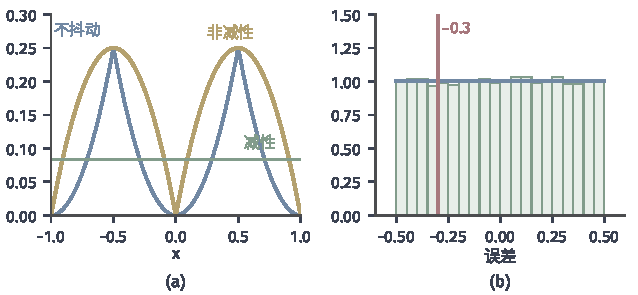
\includegraphics[width=108mm]{figures/07-probability/05-source-coding/matplotlib/quant-dither-mse/figure.pdf}
 \caption{$\Delta=1$的无穷均匀量化器在三种方式下的误差。(a) 给定读数$x$的条件均方误差：蓝线为不加抖动$(x-Q_1(x))^2$，绿线为减性抖动$\frac1{12}$，黄线为非减性抖动$s(1-s)$，$s=x-\lfloor x\rfloor$。(b) $x=0.3$时减性抖动的误差，$20000$个抖动值（种子4）的直方图（浅绿）与均匀密度（蓝线）；红线为不加抖动时的固定误差$-0.3$。}
 \label{fig:quant-dither-mse}
\end{BookInlineFigure}

图~\ref{fig:quant-dither-mse}左图把三种方式放在一起。不加抖动时，条件均方误差在刻度上为零、在刻度中点达到$\Delta^{2}/4$，形状完全由读数决定；非减性抖动消除了偏差，但条件均方误差仍随读数起伏，而且整体更大；只有减性抖动使条件均方误差与读数无关。三者的差别在于误差中有多少成分由读数决定，而这取决于解码器知道多少关于扰动的信息。


\section{本章小结}
\label{sec:quant-summary}

本章开头问：每个Laplace读数只存2个比特时，4个代表值放在哪里、读数怎样归属、平均误差多大。答案依次是：从均匀刻度出发，平均失真为$0.514$；按两条必要条件交替改进，得到阈值$\pm1.594$、重构值$\pm0.594$与$\pm2.594$，平均失真降到$0.352$；若允许变长记录，同一量化器的索引平均只需$1.805$ bit，而改用均匀刻度配合熵编码，在相近的平均长度下平均失真可以降到$0.21$左右。

\paragraph{三样东西决定三件事}
一个量化器由区域与重构值组成，它们共同决定平均失真$D(Q)$；索引的编码方式决定平均描述长度；是否加入共享的随机扰动，决定误差与读数之间的关系。三者分工不同：无损的索引编码不改变重构值，从而不改变失真；减性抖动不减小平均失真，只改变误差的结构。

\paragraph{平方误差下的两条条件}
固定区域时，最好的重构值是区域的质心，这来自平行轴恒等式~\eqref{eq:quant-parallel-axis}，也说明此时量化输出是给定索引下的条件期望；固定重构值时，最好的区域是最近邻区域，标量时阈值取中点，向量时得到Voronoi区域。最优量化器必须满足这两条，但满足它们的量化器未必最优。Lloyd--Max算法及其向量推广交替执行两步，平均失真单调不增，可能停在局部最优，结果依赖初值。

\paragraph{构造之间的比较}
本章的各种构造分别改变量化的不同环节，作用与代价各不相同。

\begin{BookInlineTable}
 \centering
 \begin{tabular}{lll}
  \toprule
  构造 & 得到什么 & 代价\\
  \midrule
  均匀量化 & 编码最简单 & 不适应分布，需饱和\\
  Lloyd--Max量化 & 按分布调整区间 & 需知道分布，局部最优\\
  向量量化 & 利用相关与形状 & 码本规模$2^{dR}$\\
  索引的熵编码 & 平均长度近$H(J)$ & 变长记录，需码表\\
  熵约束量化 & 按平均码长设计 & 目标含码长项\\
  减性抖动 & 误差独立于读数 & 共享随机数\\
  \bottomrule
 \end{tabular}
 \caption{本章各种构造的作用与代价。}
 \label{tab:quant-summary}
\end{BookInlineTable}

表~\ref{tab:quant-summary}汇总了各种构造。比较它们时，必须固定同一个源分布、同一个失真函数和同一种描述资源：重构点数、定长索引长度与平均索引长度是三种不同的预算，在一种预算下最好的方案，在另一种预算下未必最好。

\paragraph{误差的结构}
有限范围的均匀量化把误差分成两部分：范围内的舍入误差不超过半个步长，高分辨率下约为$\Delta^{2}/12$乘以范围内的概率；范围外的过载误差无界，其大小与尾部概率由读数的尾部决定。步长和范围的选择是这两部分之间的权衡，点数增加时范围也必须随之变宽。确定性量化的误差是读数的函数，“独立均匀噪声”只是高分辨率下的近似；只有在减性抖动下，它才精确成立。

\paragraph{有限方案与渐近极限}
本章的所有方案都是有限的：给定维数和点数，可以执行，也可以算出代价。它们不回答一个更根本的问题：允许把任意长的读数块放在一起描述时，给定每读数的比特数，平均失真最低能到多少。第~\ref{chap:rate-distortion}章用重构条件分布上的优化刻画这一极限，并把本章的有限量化器放到同一个标准下，衡量它们与极限之间的差距。

